%\documentclass[journal, onecolumn, letterpaper]{IEEEtran}
%\documentclass[journal,onecolumn]{IEEEtran}
% \documentclass[conference]{IEEEtran}
\documentclass[a4paper, 12pt, onecolumn,singlespacing]{article}

% The preceding line is only needed to identify funding in the first footnote. If that is unneeded, please comment it out.
\usepackage[level]{fmtcount} % equivalent to \usepackage{nth}
% \include{util}
\usepackage[portuguese, brazil]{babel}
\usepackage{multirow}
\usepackage{array} % for defining a new column type
\usepackage{varwidth} %for the varwidth minipage environment
\usepackage[super]{nth}
\usepackage{authblk}
\usepackage{cite}
\usepackage{amsmath,amssymb,amsfonts}
\usepackage{ulem}
\usepackage{graphicx}
% \usepackage{subfig}
\usepackage{textcomp}
\usepackage{xcolor}
\usepackage{mathptmx}
\usepackage{ragged2e}
\usepackage[T1]{fontenc}
\usepackage{textcomp}
\usepackage{titlesec}
\usepackage{helvet}
\usepackage{gensymb}
\usepackage{setspace} % espacamento entre linhas
\usepackage{pgfplots}
\usepackage{tikz}
\usepackage{subcaption}
\usepackage{minted}
\usepackage[left=2cm, right=2cm, bottom=2cm, top=2cm]{geometry} 
\usepackage{makecell}
\usepackage{pdfpages}
\usepackage[ISO]{diffcoeff}
\usepackage{lscape}
\usepackage{tabularx}
\usepackage{booktabs}
\usepackage{longtable}


\usepackage{fancyhdr}
\renewcommand{\headrulewidth}{1pt}
\renewcommand{\footrulewidth}{0.5pt}
\fancyhf{} % limpa os cabecalhos e rodapés
\fancyhead[C]{\textit{CURSO DE ENGENHARIA DOS RAIOS - TE981} } % define o cabeçalho personalizado
\fancyfoot[C]{\textit{AUGUSTO MATHIAS ADAMS}}
\pagestyle{fancy} % sem definir esse comando, o cabeçalho personalizado não é exibido

\renewcommand\theadalign{bc}
\renewcommand\theadfont{\bfseries}
\renewcommand\theadgape{\Gape[4pt]}
\renewcommand\cellgape{\Gape[4pt]}

%dashed line
\usepackage{booktabs, makecell}
\renewcommand\theadfont{\bfseries}
\renewcommand\theadgape{}
\usepackage{arydshln}
\setlength\dashlinedash{0.2pt}
\setlength\dashlinegap{1.5pt}
\setlength\arrayrulewidth{0.3pt}

% padrao 1.5 de espacamento entre linhas
\setstretch{1.5}
\makeatletter
\def\@maketitle{%
	\newpage
	\null
	\vskip 2em%
	\begin{center}%
		\let \footnote \thanks
		{\LARGE \@title \par}%
		\vskip 1.5em%
		{\large
			\lineskip .5em%
			\begin{tabular}[t]{c}%
				\@author
			\end{tabular}\par}%
		%\vskip 1em%
		%{\large \@date}%
	\end{center}%
	\par
	\vskip 1.5em}
\makeatother

\title{\normalsize{ENGENHARIA DOS RAIOS - TE981}\\ \huge{\textbf\textit{{Tradução de Artigo - FRACTAL MODEL OF A COMPACT INTRACLOUD DISCHARGE. I. FEATURES OF THE STRUCTURE AND EVOLUTION - D. I. Iudin and S. S. Davydenko}}\\}}
\author{\small{AUGUSTO MATHIAS ADAMS}}
\setcounter{Maxaffil}{0}
\renewcommand\Affilfont{\itshape\small}

\begin{document}
	% Seleciona o idioma do documento
	\selectlanguage{brazil}
	
	% título
	\maketitle

	\begin{abstract}
		\textit{Propomos um novo modelo de uma descarga compacta intra-nuvem, considerada como resultado da interação entre duas (ou mais) estruturas de \textit{streamer} bipolar formadas em um campo elétrico de grande escala em uma nuvem de tempestade. O modelo assume duas etapas no desenvolvimento da descarga compacta. Na etapa preliminar, duas ou mais estruturas de \textit{streamer} bipolar aparecem sucessivamente na nuvem de tempestade, na região de um campo elétrico intenso (nas fronteiras entre as regiões de cargas elétricas positivas e negativas principais ou entre a região principal de carga positiva e a camada superior de blindagem negativa). O tempo de desenvolvimento dessas estruturas é determinado pelas características dos canais condutores que as formam e pode chegar a dezenas de milissegundos. A sincronização espaciotemporal das estruturas de \textit{streamer} bipolar é proporcionada pela modulação de altitude do campo elétrico, que, em particular, pode originar-se de uma turbulência de grande escala do meio da nuvem ou da instabilidade do fluxo. É mostrado que uma única estrutura de \textit{streamer} bipolar acumula cargas elétricas significativas de sinais diferentes em suas extremidades à medida que se desenvolve. O início da etapa principal de uma descarga compacta intra-nuvem corresponde à ocorrência do canal condutor (quebra da lacuna) entre as estruturas maduras de \textit{streamer}. A carga elétrica acumulada nas extremidades adjacentes das estruturas nessa etapa é neutralizada em um tempo muito mais curto do que a duração da etapa preliminar. Os parâmetros do pulso de corrente estão em boa concordância com as estimativas da corrente de uma descarga compacta intra-nuvem obtidas na aproximação de linha de transmissão.}
	\end{abstract}

	
	\section{HISTÓRIA DOS ESTUDOS E MODELOS FÍSICOS DE DESCARGAS COMPACTAS INTRANUVEM}
	
	Os resultados de observações de descargas intra-nuvem incomuns, cujo campo elétrico na zona distante tinha a forma de um único pulso bipolar com duração de 10 a 30 $\mu s$ e acompanhado por uma explosão curta de alta potência de radiação de alta frequência, foram publicados pela primeira vez em [1]. Mais tarde, essas fontes elétricas foram classificadas como uma classe separada e denominadas descargas compactas intra-nuvem (\textit{CIDs}). Apesar dos estudos plurianuais das \textit{CIDs} e do significativo volume de dados experimentais acumulados até o momento, a natureza desse fenômeno é, em muitos aspectos, pouco clara. Neste artigo, propomos um novo modelo de descargas compactas intra-nuvem, que se baseia na abordagem fractal para a descrição de sua estrutura elétrica.
	
	\subsection{HISTÓRICO DOS ESTUDOS DE DESCARGAS COMPACTAS INTRANUVEM}
	
	Os resultados da detecção de radiação eletromagnética de descargas elétricas nas nuvens com propriedades incomuns foram publicados no início dos anos 80 do século passado [1]. A característica principal dessas descargas era uma explosão de alta potência de radiação de alta frequência nas frequências de 3 a 300 $MHz$, cujo nível excedia consideravelmente os valores das descargas intra-nuvem típicas e das descargas entre nuvem e solo. Sincronamente com a explosão de radiação de alta frequência, sensores terrestres não calibrados registraram uma variação característica no campo elétrico de baixa frequência na forma de um pulso bipolar com duração total de 10 a 20 $\mu s$ (no experimento [1], o critério para o início do pulso de campo elétrico era o excedente da intensidade de radiação do nível dado, relativamente alto, em uma frequência de 3, 139 ou 295 $MHz$). De acordo com [1], a duração de um pulso bipolar excedeu consideravelmente a duração do pulso de alta frequência registrado nas proximidades do máximo do pulso do campo elétrico, e a amplitude do pulso bipolar era cerca de 1/3 do valor de pico do campo elétrico para um retorno típico. Em tal caso, a direção do campo elétrico no primeiro semiperíodo de um pulso bipolar era oposta à direção do campo de tempo bom, ou seja, o pulso bipolar tinha uma polaridade oposta em comparação com as rajadas de campo para a descarga negativa da nuvem para o solo.
	
	Nos anos seguintes, o estudo experimental e teórico dessas descargas tem sido objeto de um número significativo de trabalhos, que proporcionaram uma visão bastante completa da radiação eletromagnética. Em particular, os autores de [2] realizaram medições de banda larga do componente de radiação do campo elétrico $E$ e sua derivada $\frac{dE}{dt}$ para dezenas de pulsos bipolares curtos e, utilizando os dados de medição de $\frac{dE}{dt}$, calcularam as densidades espectrais de energia e potência do pulso do campo elétrico. Normalizando e fazendo uma média dos pulsos bipolares de polaridade positiva (quando o campo elétrico no primeiro semiciclo do pulso é direcionado para cima para o observador em terra), os autores de [2] obtiveram os seguintes parâmetros do pulso: duração da parte inicial (positiva) do pulso em HPPW de 2,4 $\mu s$, intervalo entre os máximos do campo positivo e negativo de 11 $\mu s$, razão entre esses máximos de 8,9 e duração total de 20 a 30 $\mu s$. O valor de pico médio do campo elétrico do pulso calculado para uma distância de 100 km da descarga foi (8 $\pm$ 5,3) $V/m$ (0,72 do valor correspondente para o pulso médio do campo de retorno), e a potência de pico média da derivada do campo foi igual a (20 $\pm$ 15) $V \times (m \times \mu s)^{-1}$). Nenhuma variação no campo elétrico de fundo foi observada em um intervalo de medição de 400 $\mu s$, e o perfil da derivada do campo elétrico do pulso continha um componente considerável de ruído em comparação com o perfil correspondente para outras descargas nas nuvens. Em [2], foram detectados pulsos curtos de ambas as polaridades (os pulsos positivos predominaram), mas não foi observada uma dependência significativa da forma do pulso em relação à polaridade do pulso. A análise quantitativa do espectro de energia do campo elétrico de pulsos bipolares mostrou que, em frequências de centenas de $kHz$ a 8 $MHz$, esse espectro é comparável ao espectro de radiação de um típico pulso de retorno, mas já em uma frequência de 18 $MHz$, na qual o espectro de radiação do pulso de retorno diminui para o nível de ruído, o espectro dos pulsos bipolares curtos o excede em 16 dB, estendendo-se acima de 50 $MHz$. Assim, em [2], a conclusão de [1] de que essas descargas são a fonte mais poderosa de radiação de alta frequência nas nuvens de tempestade foi confirmada. Medições de banda larga dos pulsos bipolares do campo elétrico em frequências de 3 a 50 $MHz$ também foram apresentadas em [3], onde foi constatado que os pulsos de polaridades positiva e negativa têm durações diferentes e não há correlação temporal dos pulsos de polaridade positiva e negativa com qualquer atividade de relâmpago conhecida na nuvem.
	
	Logo após a publicação dos dados de medição realizados em solo mencionados em [4-6], mais de 500 pares de pulsos incomuns de radiação de alta frequência foram registrados a bordo do satélite ALEXIS. A dispersão dos pares de explosões, claramente visível em seus espectros dinâmicos, indicou que sua fonte está localizada sob a ionosfera. Portanto, em [4, 5], tais explosões foram chamadas de pares de pulsos transionosféricos (\textit{TIPPs}, na sigla em inglês). De acordo com [4, 5], na faixa de 28 a 95 $MHz$, os pares de pulsos transionosféricos são explosões de radiação com duração de 1 a 20 $\mu s$ (com duração média de 2 a 4 $\mu$s), separadas por um intervalo de tempo de 10 a 100 $\mu s$ (com intervalo médio de 50 $\mu$s). A intensidade do pulso excedeu em 20 a 40 dB o nível de fundo, e a potência do pulso nessa faixa foi pelo menos uma ordem de magnitude maior do que a potência irradiada de uma descarga típica de raios. Na faixa de 117 a 166 $MHz$, as características estatísticas dos pares de pulsos transionosféricos diferiram apenas ligeiramente em relação às características na parte inferior da faixa de frequência muito alta (\textit{VHF}, de 30 a 300 $MHz$), exceto pela diminuição na dispersão e atraso médio entre os pulsos, que foi de 37 $\mu$s [6]. Tanto na parte de baixa frequência quanto na parte de alta frequência da faixa \textit{VLF}, durante o registro de um par de pulsos (com duração de registro de 7 a 100 $ms$), a radiação de descargas de raios não foi observada como regra geral. Os autores de [4-6] fizeram duas suposições sobre a origem dos pares de pulsos. A primeira suposição foi que o segundo pulso é a reflexão da radiação de uma fonte pulsada de alta altitude a partir da superfície da Terra. A segunda suposição é que ambos os pulsos são irradiados por fontes diferentes, mas correlacionadas, cuja conexão não está clara.
	
	A gravação de pares de pulsos subionosféricos (\textit{SIPPs}) na faixa de alta frequência (\textit{HF}, de 3 a 30 $MHz$) durante observações em solo não esclareceu a origem e a natureza do segundo pulso [7]. Uma vantagem das observações em solo foi a determinação mais precisa da posição da fonte: o raio da região de sua possível localização variou de 300 a 520 $km$, à medida que a altitude da fonte variou de 5 a 15 $km$, sendo muito menor que o raio da área de vigilância do \textit{ALEXIS}, que era de 3000 $km$. Isso levou à conclusão de que cerca de 350 pares de pulsos subionosféricos dos 500 observados correspondiam a regiões de atividade de tempestades próximas, e em outros casos a atividade de tempestades foi observada a uma distância de até alguns milhares de quilômetros. Além disso, todos os pares de pulsos subionosféricos foram registrados no período de 20:00 às 04:00 LT, o que também indica sua relação com as tempestades regionais. As características dos pares de pulsos subionosféricos e transionosféricos eram semelhantes, exceto pela ausência de dispersão e divisão de modos nas observações em solo da maioria dos eventos. A comparação das características de dispersão da radiação refletida na ionosfera de uma descarga de raio remota e sete pares de pulsos subionosféricos registrados com dispersão permitiu aos autores concluir sobre a localização próxima (não mais do que algumas dezenas de quilômetros) de suas fontes e da nuvem de tempestade. Em geral, de acordo com [7], a gravação de pares de pulsos subionosféricos é evidência da existência de uma fonte separada para o segundo pulso, uma vez que nas observações em solo a presença do segundo pulso não pode ser explicada pela reflexão do pulso inicial da superfície terrestre.
	
	Características importantes de pulsos bipolares curtos foram obtidas em [8] com base nos dados de dois sistemas multiponto de registro do campo elétrico e radiação de alta frequência na faixa de 3 a 30 $MHz$. Nesse caso, as características de ajuste do sistema de disparo dos sensores permitiram o registro apenas dos pulsos de polaridade positiva. Além das características médias (ao longo de 24 eventos) dos pulsos bipolares curtos do campo elétrico e das respectivas rajadas de radiação de \textit{HF} para três tempestades no Novo México e Texas (EUA; ver Tabela 1), a localização da fonte de radiação foi determinada pela primeira vez nesse artigo. A distância até a fonte foi determinada pelo tempo de atraso do sinal nas estações espacialmente separadas, e a altitude da fonte, pelo atraso na chegada dos sinais refletidos pela ionosfera e pela Terra e ionosfera em relação ao pulso que se propaga sem reflexões, pela distância mais curta. Como resultado, verificou-se que as fontes de pulsos bipolares estão localizadas em nuvens de tempestade a altitudes de 8 a 11 km acima do nível do mar, próximas a regiões com nível de reflexão do sinal de radar acima de 40 $dBZ$. Assim como nos estudos anteriores, os autores de [8] observaram nenhuma correlação entre pulsos bipolares curtos e qualquer atividade conhecida de raios na nuvem e relataram que os pulsos bipolares eram quase sempre o único evento no intervalo de 5 a 50 $ms$. O mesmo é verdade para a rajada de radiação de \textit{HF}.
	
	\begin{longtable}{@{}p{12cm}c@{}}
		\caption{Características médias de pulsos bipolares curtos do campo elétrico e explosões síncronas de radiação de alta frequência na faixa de 3--30 $MHz$, de acordo com [8].} \l\label{tabela1}\\
			\toprule
			\multicolumn{2}{c}{\textbf{Características  do Campo Elétrico de Pulsos Bipolares Curtos}} \\
			\midrule
			Tempo de subida do campo (de 10\% a 90\% do máximo), $\mu$s & $2.3 \pm 0.8$ \\
			Duração da rajada inicial do campo elétrico (no nível do meio pico), $\mu$s & $4.7 \pm 1.3$ \\
			Duração total do pulso, $\mu$s & $25.8 \pm 4.9$ \\
			Valor de pico do campo elétrico na rajada inicial (primeiro) de um pulso bipolar (a uma distância de 100 km da fonte), V/m & $9.5 \pm 3.6$ \\
			Valor de pico do campo elétrico na segunda rajada de um pulso bipolar (a uma distância de 100 km da fonte), V/m & $-3.9 \pm 1.6$ \\
			Razão das amplitudes de pico do campo elétrico na primeira e segunda rajadas de um pulso bipolar & $2.7$ \\
			Razão das amplitudes de pico do campo elétrico de um pulso bipolar e do pulso devido ao retorno do raio & $0.71$ \\
			Razão das amplitudes de pico do campo elétrico de um pulso bipolar e do pulso devido à descarga intra-nuvem & $2.6$ \\
			\midrule
			\multicolumn{2}{c}{\textbf{Características da Radiação de Alta Frequência}} \\
			\midrule
			Duração, $\mu$s & $2.8 \pm 0.8$ \\
			Valor de pico do campo (a uma distância de 10 km na faixa de 1 kHz), mV/m & $2.4 \pm 1.1$ \\
			Razão das amplitudes de pico do campo de alta frequência de uma descarga compacta intra-nuvem e do \textit{Return Stroke} & $9.9$ \\
			Razão da amplitude de pico do campo de alta frequência de descargas compactas e convencionais intra-nuvem & $29$ \\
			\bottomrule
	\end{longtable}

	Como resultado da comparação dos dados acima sobre a rajada de radiação de HF que é síncrona com um pulso bipolar curto do campo elétrico e os parâmetros dos pares de pulsos transionosféricos, os autores de [8] chegaram à conclusão de que o fenômeno físico é o mesmo. O segundo pulso transionosférico é a reflexão do pulso inicial da superfície da Terra, o que proporciona uma interpretação natural dos diferentes atrasos entre os pulsos nas diferentes faixas de frequência [4-6]. O ponto é que as observações dos pares de pulsos na parte inferior da faixa \textit{VLF} foram realizadas sobre regiões equatoriais (ver [4, 5]), e na parte superior da faixa \textit{VLF}, sobre o território dos EUA (ver [5]), onde a altitude das nuvens de tempestade é menor do que perto do equador. Se a fonte de pulsos \textit{VLF} estiver localizada nas proximidades do topo de uma nuvem de tempestade, então o atraso entre os pulsos é diferente nesses casos. Essa suposição também explica a situação comum em que a intensidade do segundo pulso no par é maior do que a do primeiro pulso (ver [4, 5]), o que pode ser devido ao padrão de diretividade não homogêneo da fonte.
	
	Uma vez que os pulsos bipolares curtos do campo elétrico em [8] foram registrados exclusivamente na zona distante, seus parâmetros podem ser convenientemente usados para a estimativa das características da fonte correspondente. De acordo com [8], a variação média do momento dipolar da fonte de pulsos bipolares foi de $0,38 C·km$, com valores mínimos e máximos de $0,26$ e $0,8$ $C·km$, respectivamente. A corrente média da fonte variou entre algumas dezenas e algumas centenas de quiloampères, à medida que a escala espacial da fonte variou de 300 a 1000 m, e a velocidade de propagação do pulso da corrente da fonte pode ser próxima à velocidade da luz. Levando em consideração as características únicas da emissão de rádio e os tamanhos relativamente pequenos dessas fontes, os autores de [9] sugeriram classificá-las como uma classe separada, denominada descargas compactas intra-nuvem (\textit{CIDs}).
	
	Os resultados importantes sobre a natureza das \textit{CIDs} foram obtidos utilizando o \textit{LMA} (\textit{Lightning Mapping Array}), um sistema terrestre de vários pontos para registro da radiação VHF de descargas de raios, localizado no Novo México (EUA). O sistema não conseguia determinar a forma e a duração de um pulso de radiação \textit{HF}, mas localizava a fonte com uma precisão de até algumas centenas de metros pelo atraso da chegada do pulso nos pontos de medição [10]. Com base nos dados do \textit{LMA}, descobriu-se que as descargas compactas intra-nuvem positivas estão localizadas entre as regiões das principais cargas positivas e negativas e, ao contrário das observações anteriores, estão sempre associadas à descarga inicial de uma descarga intra-nuvem convencional. Nesse caso, a maioria das descargas intra-nuvem se desenvolveu sem a ocorrência de \textit{CIDs} na fase inicial. De acordo com [10], as fontes de radiação VLF de alta potência das \textit{CIDs} estavam distribuídas na região com uma escala típica de algumas centenas de metros a um quilômetro e, ao contrário das descargas de raios convencionais, não eram descritas por um conjunto de fontes pontuais. Estimativas [10, 11] mostraram que a potência da radiação CID na faixa de 60-66 $MHz$ poderia atingir $300 kW$ e é mais de uma ordem de grandeza maior do que a potência radiada da descarga intra-nuvem subsequente, que não ultrapassa 10 $kW$.
	
	As possibilidades de registrar a radiação das descargas compactas intra-nuvem se tornaram muito mais amplas com o lançamento do satélite \textit{FORTE} em 1997 [12]. Os receptores do satélite registravam a radiação nas frequências de 26 a 48 $MHz$ simultaneamente para duas polarizações diferentes ou a radiação de uma polarização simultaneamente nas faixas de 26-48 e 118-140 $MHz$. Além disso, sensores ópticos de alta sensibilidade foram instalados a bordo do satélite. O registro por satélite de pares de pulsos transionosféricos no caso em que a localização da descarga não é conhecida permitiu determinar a relação entre as altitudes das fontes de diferentes eventos [12], e a altitude da descarga se os dados de coordenadas geográficas da descarga estiverem disponíveis [13], assumindo que o segundo pulso é o reflexo do primeiro pulso na superfície da Terra. As coordenadas geográficas da descarga foram determinadas, em particular, a partir dos dados do registro do campo elétrico na faixa VLF/HF (nas frequências de 3 a 300 kHz) pelos sistemas de vários pontos LASA (\textit{Los Alamos Sferic Array}) [14] e NLDN (\textit{National Lightning Detection Network}) [15].
	
	A análise dos dados de medição terrestre e por satélite da radiação de descargas compactas permitiu determinar sua localização, altitude e brilho óptico. Em primeiro lugar, foi demonstrado, com precisão na determinação da localização do satélite \textit{FORTE}, que as fontes de um pulso bipolar curto do campo elétrico e pares de pulsos transionosféricos coincidem no espaço e no tempo nos casos de registro combinado dos eventos nas faixas \textit{VLF/LF} e \textit{HF/VHF} [16, 17]. Verificou-se que os pares de pulsos transionosféricos de alta frequência, com potência efetiva superior a 40 $kW$ na faixa de 26 a 48 $MHz$ e duração de 3 a 5 $mu s$, são fracamente polarizados, incoerentes, observados separadamente de outros fenômenos ou iniciam uma descarga intra-nuvem, cuja radiação na faixa de VHF é muito mais fraca do que a radiação \textit{CID} [16, 18]. Quando a radiação \textit{CID} é registrada simultaneamente nas faixas de baixa frequência (\textit{LASA}) e alta frequência (\textit{FORTE}), constatou-se que o número de pares de pulsos transionosféricos excede o número de pulsos de campo elétrico bipolar curto. O pulso de radiação CID de uma descarga compacta, regra geral, não é acompanhado do componente de baixa frequência no caso em que o \textit{CID} inicia uma descarga intra-nuvem e o desenvolvimento do líder. Se o pulso de alta frequência é acompanhado pela formação de um pulso de campo elétrico bipolar curto, então, inversamente, a descarga intra-nuvem não se desenvolve [18]. Independentemente da formação do pulso de campo elétrico bipolar, as descargas compactas intra-nuvem irradiam de forma relativamente fraca na faixa óptica em comparação com as descargas de raios convencionais [19, 20]. Entre os resultados recentes das observações por satélite da radiação \textit{CID}, mencionamos o artigo [21], no qual foram observadas diferenças específicas dos pulsos transionosféricos diretos e refletidos pela Terra em uma frequência de 130 $MHz$, e o efeito ionosférico pôde ser negligenciado.
	
	O padrão de radiação de alta frequência das \textit{CIDs} obtido por meio de experimentos realizados em satélite é complementado de forma natural com os resultados do registro da radiação \textit{CID} por sistemas terrestres. Isso ocorre porque algumas características das \textit{CIDs}, em particular a polaridade e a estrutura espacial detalhada, só podem ser determinadas pelo registro do campo elétrico terrestre. Como principais resultados das observações terrestres de \textit{CIDs} obtidas nos últimos anos, mencionamos o seguinte. Em [17], com base na análise de quase 100.000 pulsos bipolares curtos registrados pelo sistema \textit{LASA}, verificou-se que as descargas compactas de polaridade diferente aparecem em altitudes diferentes. A altitude média acima da superfície da Terra para as \textit{CIDs} positivas e negativas foi de 13 $km$ (para a faixa de altitudes de descarga de 7 a 15 km) e 18 $km$ (para a faixa de altitudes de descarga de 15 a 20 $km$), respectivamente, e a proporção entre o número de descargas positivas e negativas foi de 58:42. As diferentes altitudes de início das \textit{CIDs} de polaridade positiva e negativa correspondem às regiões com diferentes direções do campo elétrico intra-nuvem. Mais especificamente, a faixa inferior de altitudes corresponde ao limite das regiões das principais cargas negativas e positivas, e a faixa superior corresponde ao limite das regiões da principal carga positiva e da camada de blindagem negativa.
	
	Os autores do artigo [22] apresentaram as primeiras (e únicas até agora) estimativas do momento de carga das \textit{CIDs}, com base nos registros do campo elétrico de sete descargas compactas na zona próxima. De acordo com [22], o momento de carga das \textit{CIDs} variou entre $0,15$ e $2$ $C·km$, com um valor médio de cerca de $1$ $C·km$. Os autores do artigo [23] analisaram a correlação entre a taxa de ocorrência de \textit{CIDs} e as descargas convencionais de raios, bem como a taxa de convecção nas nuvens de tempestade sobre as Grandes Vales (EUA) de maio a julho de 2005. A comparação dos dados do \textit{LASA} e do \textit{NLDN} com os resultados do radar mostrou o seguinte. Em primeiro lugar, verificou-se que a taxa de ocorrência de \textit{CIDs} apresenta uma correlação fraca com a taxa de convecção na nuvem de tempestade e a taxa de ocorrência das descargas convencionais de raios. Por um lado, nas nuvens com convecção fraca, as descargas compactas não foram detectadas, enquanto nas nuvens com \textit{CIDs}, ao contrário, sempre houve uma convecção intensa (em particular, para essas nuvens, a região com nível de reflexão do sinal de radar superior a 30 $dBZ$ estava localizada 4-5 $km$ acima, e o máximo do nível de reflexão era de 10-13 $dB$ mais alto do que para as descargas convencionais de raios). Por outro lado, as \textit{CIDs} não puderam ocorrer nas células de tempestade com a convecção mais intensa. Uma característica importante das descargas compactas foi o agrupamento espaço-temporal. Ou seja, a maioria das \textit{CIDs} foi registrada em várias tempestades intensas (em particular, 34\% de todas as \textit{CIDs} foram detectadas na frente de nuvens de tempestade intensas durante 11 horas em 24-25 de maio de 2005). Também foi constatado que o número de \textit{CIDs} não excede 0,5\% do número total de descargas de raios. As \textit{CIDs} de ambas as polaridades puderam ser registradas em uma única nuvem, sendo que o número de \textit{CIDs} positivas correspondia a aproximadamente 77\% de todas as descargas compactas registradas.
	
	As conclusões sobre o efeito da taxa de convecção no desenvolvimento das \textit{CIDs} e na predominância das descargas compactas positivas, obtidas em [23], geralmente estão em conformidade com os resultados de medições em outras regiões e condições climáticas (consulte, em particular, [14, 24–26]). No entanto, a taxa de ocorrência de \textit{CIDs} em relação ao número total de descargas de raios varia drasticamente dependendo da latitude geográfica das observações, variando de mais de 3\% na Flórida (EUA) [14, 24] a 0,034\% no norte da China [25], chegando à ausência total na Suécia [26]. A análise das observações das \textit{CIDs} positivas na Flórida (EUA) confirmou sua natureza predominantemente isolada, com aproximadamente 73\% dos eventos não estando relacionados às descargas convencionais de raios. Pares de descargas compactas (cerca de 4\% dos eventos), separados por um intervalo de tempo de 43 a 181 ms [27], foram registrados pela primeira vez lá. Em [28], com base nos registros de 244 pulsos bipolares positivos curtos do campo elétrico, foi sugerido categorizá-los por forma (o "clássico" pulso bipolar suave foi observado apenas em 5\% dos casos). Também foi observado em [28] que as \textit{CIDs} são geralmente isoladas no espaço e no tempo em relação a outras descargas na nuvem, enquanto as altitudes das \textit{CIDs} correspondem bem aos resultados de [17]. Uma análise comparativa das propriedades das \textit{CIDs} positivas e negativas com base nos dados de medição do campo elétrico \textit{VLF/LF} é apresentada em [29], onde, além das diferentes altitudes de localização das \textit{CIDs} de polaridade diferente, foi observado que as \textit{CIDs} negativas, em geral, não apresentam uma maior amplitude do pulso bipolar do campo elétrico e estão mais separadas no tempo. Também foi mencionado que, apesar do maior número médio de \textit{CIDs} positivas, a taxa de ocorrência das descargas compactas negativas foi maior em alguns intervalos de tempo do que a das positivas.
	
	\subsection{MODELOS FÍSICOS DE DESCARGAS COMPACTAS INTRA-NUVEM (CID)}
	
	Uma das primeiras suposições sobre a natureza das \textit{CIDs} foi feita em [1], onde foi sugerido que os surtos de radiação observados podem ser interpretados como consequência do processo K muito rápido. No entanto, os tempos característicos de variação do campo elétrico nos processos \textit{K} (cerca de 1 ms) excedem em muito as escalas de tempo das \textit{CIDs}, e essas variações geralmente têm a forma de uma sequência de saltos separados por 10 a 30 ms [30], em contradição com a natureza predominantemente singular dos surtos de campo elétrico de baixa frequência para \textit{CIDs}. Além disso, as descargas de campo elétrico de milissegundos que são típicas dos processos K não são observadas para as \textit{CIDs}, e a potência da radiação VHF excede em ordens de grandeza o valor correspondente para os processos \textit{K} [31, 32]. Nesse sentido, a interpretação proposta em [1] para as \textit{CIDs} não é satisfatória.
	
	Outro modelo para a ocorrência da descarga compacta é baseado no mecanismo de quebra por elétrons em fuga [33, 34]. Esse mecanismo baseia-se no fato de que a força de desaceleração de um elétron no meio é inversamente proporcional à sua energia. Portanto, na presença de um campo elétrico externo que excede algum valor limite, um elétron semente energético pode ser constantemente acelerado e adquirir energia suficiente para ionizar moléculas neutras. Como resultado, surgem os chamados elétrons secundários no meio. Parte deles possui alta energia e também pode se tornar elétrons em fuga. A avalanche resultante de elétrons em fuga e um grande número de elétrons secundários lentos pode alterar drasticamente a condutividade do meio e levar a uma quebra elétrica [35]. A fonte de elétrons semente são os raios cósmicos, cuja energia determina, em muitos aspectos, a forma do pulso de corrente formado e a emissão eletromagnética de banda larga da avalanche de elétrons.
	
	De fato, foi demonstrado em [36] que, dentro de uma descrição simplificada da avalanche de elétrons como uma carga pontual crescente se movendo verticalmente com velocidade constante, é possível obter um bom acordo entre os resultados do cálculo e as medições do campo elétrico no solo em diferentes distâncias da descarga. A melhor coincidência é alcançada no caso em que a fonte não é uma, mas um conjunto de avalanches de elétrons surgindo em um ponto com uma probabilidade dada em algum intervalo de tempo. No entanto, a interpretação detalhada da radiação das \textit{CIDs} dentro da teoria de quebra por elétrons em fuga encontra certas dificuldades. Algumas delas são discutidas em [37], onde, no exemplo de três pulsos de campo elétrico \textit{CID} bipolares registrados, foi mostrado que para sua geração, a quebra por elétrons em fuga deve ter parâmetros extremos. Em primeiro lugar, a partícula iniciadora da quebra dos raios cósmicos deve ter uma energia de cerca de $1021$ $eV$, o que excede o limite de \textit{Greisen-Zatsepin-Kuz'min} [38]. Essa circunstância diminui abruptamente a probabilidade de tal quebra. De fato, de acordo com [37], uma partícula com a energia correspondente entra em uma nuvem com uma área de 100 $km^2$ uma vez a cada 67 anos. Além disso, nos exemplos considerados, de acordo com [37], o canal condutor tem de 8 a 13 $km$ de comprimento e a corrente de descarga excede 500 $kA$, o que excede em muito as estimativas dos parâmetros de \textit{CIDs} obtidas em termos do modelo de linha de transmissão (ver, por exemplo, [39]). A própria quebra deve se desenvolver em um campo elétrico intra-nuvem que excede várias vezes o valor crítico em uma considerável faixa de altitudes, mas isso nunca foi observado nas nuvens de tempestade reais. No que diz respeito à interpretação da radiação \textit{CID} de alta frequência dentro do mecanismo de quebra por elétrons em fuga, os problemas que surgem nesse caso se devem à duração pequena (\textit{submicrossegundos}) e ao padrão de direção estreita do surto de radiação de HF, bem como a uma potência radiada insuficiente na parte superior da faixa \textit{VLF} [40]. A avalanche de elétrons que fornece um nível aceitável de radiação de alta frequência dentro do modelo [40] forma um pulso de campo elétrico bipolar que não está de acordo com as observações. O feixe estreito da radiação de quebra por elétrons em fuga não permite explicar as observações de satélite dos pares de pulsos transionosféricos, e a suposição proposta em [41] sobre a iniciação de duas quebras por uma partícula energética em altitudes diferentes (acima da nuvem de tempestade e na mesosfera) não foi confirmada experimentalmente. Também observamos que as estimativas apresentadas em [42] em relação ao aumento da condutividade do meio intra-nuvem devido à geração de elétrons secundários questionam o próprio mecanismo de quebra por elétrons em fuga.
	
	Com base no que foi dito acima, pode-se concluir que, atualmente, não há um modelo físico autoconsistente de descargas compactas intra-nuvens (\textit{CIDs}). Neste artigo, propomos um novo mecanismo para a iniciação de \textit{CIDs}, que se baseia na abordagem fractal para descrever descargas elétricas intra-nuvens. Uma descarga compacta intra-nuvem é considerada como resultado da interação de duas estruturas bipolares de \textit{streamer} que se desenvolvem em um campo elétrico externo não uniforme em larga escala. Na primeira parte deste trabalho, consideramos as características do surgimento e evolução das \textit{CIDs}. Na segunda parte, discutimos a radiação das \textit{CIDs} em diferentes faixas de frequência, de acordo com o modelo proposto.
	
	\section{O MODELO DE UMA DESCARGA COMPACTA INTRANUVEM}
	
	A modelagem das \textit{CIDs} está intimamente relacionada a uma das características básicas da descarga elétrica nas nuvens de tempestade, ou seja, a combinação da baixa condutividade estática do meio intra-nuvem e a rápida coleta observada (de algumas dezenas de microssegundos no caso de uma \textit{CID} a centenas de milissegundos nas descargas convencionais de raios) da carga elétrica de uma parte considerável da nuvem de tempestade para o canal de descarga. Os autores [44–47] propuseram um mecanismo de coleta de carga baseado na formação de um sistema de canais condutores na nuvem, que efetivamente desempenham o papel de um sistema de drenagem elétrica. Em termos gerais, tal sistema de condutores deve incluir elementos com tamanhos variando das distâncias entre partículas carregadas à escala da nuvem de tempestade, o que torna sua descrição completa extremamente difícil. Nesse sentido, todos os modelos existentes de alguma forma limitam o nível de detalhes espaciais na descrição da descarga, geralmente omitindo os processos microfísicos e fenômenos em pequena escala. Em todos os artigos mencionados, os autores consideraram como o elemento condutor a parte da descarga líder cujo desenvolvimento foi descrito dentro da equação de \textit{Poisson} tridimensional com o campo elétrico externo e o modelo estocástico de quebra dielétrica, proposto anteriormente em [44, 48, 49]. Com algoritmos um tanto diferentes em detalhes, todos esses modelos têm duas restrições significativas. Primeiramente, eles não permitem o crescimento simultâneo de diferentes ramos da descarga e, em segundo lugar, a escala temporal está ausente neles, resultando em que os ramos da descarga não transportam correntes. A primeira dessas restrições foi superada em [50], onde um modelo de percolação da descarga de raios baseado em uma rede de autômatos celulares foi proposto dentro do paradigma da crítica auto-organizada. Em seguida, as correntes da árvore de descarga foram levadas em conta dentro da mesma abordagem [51, 52], o que permitiu calcular as características da radiação de alta frequência da descarga de raios. No presente artigo, também usamos abordagens baseadas no modelo de autômatos celulares para descrever uma descarga compacta intra-nuvem. Como elemento (célula) do modelo, consideramos o volume cúbico do meio da nuvem, que pode conter uma carga elétrica total. O tamanho de uma célula elementar excede em muito a distância entre os portadores de carga física, ou seja, as partículas da nuvem cujo carregamento pode ser fornecido por vários mecanismos de eletrização [53] e alguns tipos de instabilidades [54, 55] na nuvem de tempestade. Ligações elétricas (condutoras) entre os elementos vizinhos são estipuladas pela iniciação de uma descarga elétrica entre eles, com a carga elétrica fluindo ao longo do canal condutor deste último. Na modelagem macroscópica, assume-se que apenas parte do volume da célula elementar está envolvida na transferência de carga. Isso se deve à suposição de que ligações de pequena escala, relativamente bem condutoras dentro de cada célula (por exemplo, estruturas de \textit{streamer}) abrangem apenas parte dos portadores. Caso contrário, toda a nuvem de tempestade seria permeada por ligações condutoras, o que poderia ter alterado drasticamente o desenvolvimento das descargas elétricas nelas.
	
	Agora consideramos as diferenças fundamentais do modelo proposto em relação aos modelos anteriores. A primeira diferença diz respeito à morfologia da descarga. Conforme mencionado anteriormente, um curto e intenso surto de radiação \textit{CID} não está de acordo com os parâmetros de uma descarga intra-nuvem convencional, que dura muito mais tempo e cuja emissão é muito mais fraca tanto nas faixas de baixa frequência quanto nas faixas de alta frequência. Dentro dos mecanismos conhecidos, não podemos explicar por que a intensidade da corrente de origem necessária para essa radiação é comparável à corrente de retorno na descarga entre nuvem e solo (veja, por exemplo, [39]). Nesse sentido, assumimos que uma descarga compacta intra-nuvem inclui duas etapas, preliminar e principal. Na etapa preliminar, duas descargas bipolares, semelhantes em forma às descargas intra-nuvem, se desenvolvem a uma distância relativamente curta uma da outra ao longo do campo elétrico externo. Cada descarga existe muito mais tempo do que o surto de radiação \textit{CID} e, ao longo de sua existência, acumula uma carga significativa de polaridades diferentes em suas extremidades opostas (na coroa e na raiz da descarga). A segunda etapa da descarga principal começa quando as coroas com cargas opostas dessas descargas entram em contato elétrico à medida que crescem. Surge um canal de corrente conectando as regiões com sinais opostos de carga, fazendo com que a carga acumulada na etapa preliminar se esgote ao longo do canal condutor emergente em um curto período de tempo. A segunda característica do modelo proposto é devida à necessidade de fornecer um nível muito baixo de radiação eletromagnética tanto nas faixas de \textit{VLF/LF} quanto nas faixas de \textit{HF/VHF} na etapa preliminar da \textit{CID}. Para isso, assumimos que na etapa preliminar, o acoplamento elétrico entre as células elementares é uma descarga do tipo \textit{streamer}, com correntes relativamente fracas e principalmente variando lentamente, correspondendo a uma radiação eletromagnética fraca (a radiação \textit{CID} será discutida em mais detalhes na segunda parte do trabalho). Observe que nas altitudes em que ocorrem as CIDs, o comprimento, a velocidade e as correntes das descargas do tipo \textit{streamer} podem variar amplamente nas regiões de campo elétrico intenso [56, 57].
	
	Consideremos com mais detalhes a eletrodinâmica das \textit{CIDs} dentro do contexto da abordagem proposta.
	
	\section{DESCRIÇÃO DE UMA ÚNICO \textit{STREAMER} DE DESCARGA BIPOLAR}
	
	Considere primeiro a dinâmica de uma descarga de \textit{streamer} bipolar única em uma região de $500 \times 500 \times 500$ m localizada nas proximidades do máximo local de um campo elétrico intra-nuvem. Para definição, consideramos os processos próximos à fronteira entre as camadas principais de carga positiva e a camada superior (negativa) de blindagem da carga espacial, onde, de acordo com observações, ocorrem os CIDs negativos. Nesse caso, negligenciamos a diferença na dinâmica e nas propriedades dos \textit{streamers} positivos e negativos, assumindo que suas velocidades são idênticas e iguais a $5 \times 10^5$ m/s [56]. O tamanho de uma célula elementar será assumido como igual a $10 \times 10 \times 10$ m, e o comprimento da ligação condutora entre células vizinhas é da ordem de 10 m. Esse valor, em termos gerais, é bastante grande para o comprimento de um único \textit{streamer}, mesmo considerando a queda de pressão nas altitudes consideradas. No entanto, pode-se supor que o acoplamento elétrico entre as células seja realizado por meio de um conjunto de \textit{streamers} ou uma estrutura de baixa corrente, semelhante aos \textit{stalkers} recentemente descobertos [58]. Além disso, as características do acoplamento elétrico podem se desenvolver como resultado de múltiplas passagens da descarga de \textit{streamer} sobre o mesmo volume. O intervalo de tempo do modelo do sistema é igual a $\tau = 20 \mu$s e é determinado pelo tempo de criação da ligação condutora entre as células vizinhas, ou seja, pela relação entre o tamanho da célula $a = 10$ m e a velocidade do \textit{streamer}.
	
	Cada célula elementar $i$ no domínio de simulação corresponde à carga elétrica acumulada $q_i$ nela. A distribuição de carga nas células no tempo inicial $t = 0$ é dada pela distribuição do campo elétrico intra-nuvem $E(\mathbf{r}, t = 0)$, que será considerado vertical. Como a região considerada é pequena em comparação com o tamanho da nuvem de tempestade, a distribuição inicial do campo pode ser assumida unidimensional: $E(\mathbf{r}, t = 0) = z_0 E_0(z)$, onde $z_0$ é o vetor unitário do eixo vertical $z$. Nesse caso, a distribuição inicial da densidade de carga na nuvem depende da coordenada vertical: $\rho(z, t = 0) = \varepsilon_0 \frac{\partial E_0(z, t)}{\partial z}$, onde $\varepsilon_0$ é a constante elétrica. A carga na célula elementar $i$, centrada no ponto de coordenada $\mathbf{r}i = (r{\perp i}, z_i)$, é igual a $q_i = a^3 \rho(z_i, t = 0)$. Para estimar o perfil inicial do campo na fronteira das camadas principais de carga positiva e a camada superior de blindagem, pode-se usar dados de sondagem de balão em nuvens de tempestade. Esses dados sugerem que nas proximidades da camada de blindagem, que varia de algumas centenas de metros a mais de um quilômetro de espessura e está localizada em altitudes de 8 a 15 km acima do nível do mar, a intensidade do campo elétrico pode atingir 50 $kV/m$ [59,60]. Sem entrar em detalhes sobre a formação da camada de blindagem (veja, por exemplo, [61,62]), assumimos, para cálculos, que o campo elétrico entre as camadas principais de carga positiva e a camada superior de blindagem é máximo a uma altitude de 12 $km$ e atinge 30 $kV/m$; a região de campo elétrico forte tem cerca de 500 $m$ de espessura.
	
	A dinâmica da carga elétrica em cada célula é determinada pela presença e estado do acoplamento elétrico com as células vizinhas. Assumimos que a probabilidade de ocorrência da descarga do \textit{streamer} (ruptura) entre as células vizinhas $i$ e $j$ depende da diferença de seus potenciais e é descrita pela distribuição de \textit{Weibull}:
	
	\begin{equation}
		P_{ij} = \begin{cases}
					1 - exp \left( -\left| \frac{E_{ij} - E_i}{E_s - E_i} \right|^m\right ), &  E_{ij} \geq E_i \\ 
					0, & E_{ij} < E_i 
				 \end{cases}
		\label{eqn_1}
	\end{equation}
	
	Aqui, $m$ é o índice de \textit{Weibull}, $E_{ij} = |\phi_i - \phi_j |/L_{ij}$, $\phi_i$ e $\phi_j$ são os potenciais elétricos das $i$-ésima e $j$-ésima células, respectivamente, $L_{ij}$ é a distância entre as $i$-ésima e $j$-ésima células, e $E_s$ e $E_i$ são os campos crítico e de iniciação do \textit{streamer}, respectivamente, tal que $E_s > E_i$. Note que sob condições de laboratório (comprimento da ordem de metros), o campo é da ordem de 100 $kV/m$ [56] e pode ser muito menor sob condições de descargas em nuvens [63]. A razão física para o aumento local (em pequena escala em comparação com o tamanho da célula) do campo e, consequentemente, a diminuição dos campos $E_s$ e $E_i$ na escala da célula em comparação com os valores de laboratório pode ser irregularidades naturais em pequena escala da densidade de carga [64]

	\begin{figure}
		
		\begin{minipage}{0.45\textwidth}
			\centering
			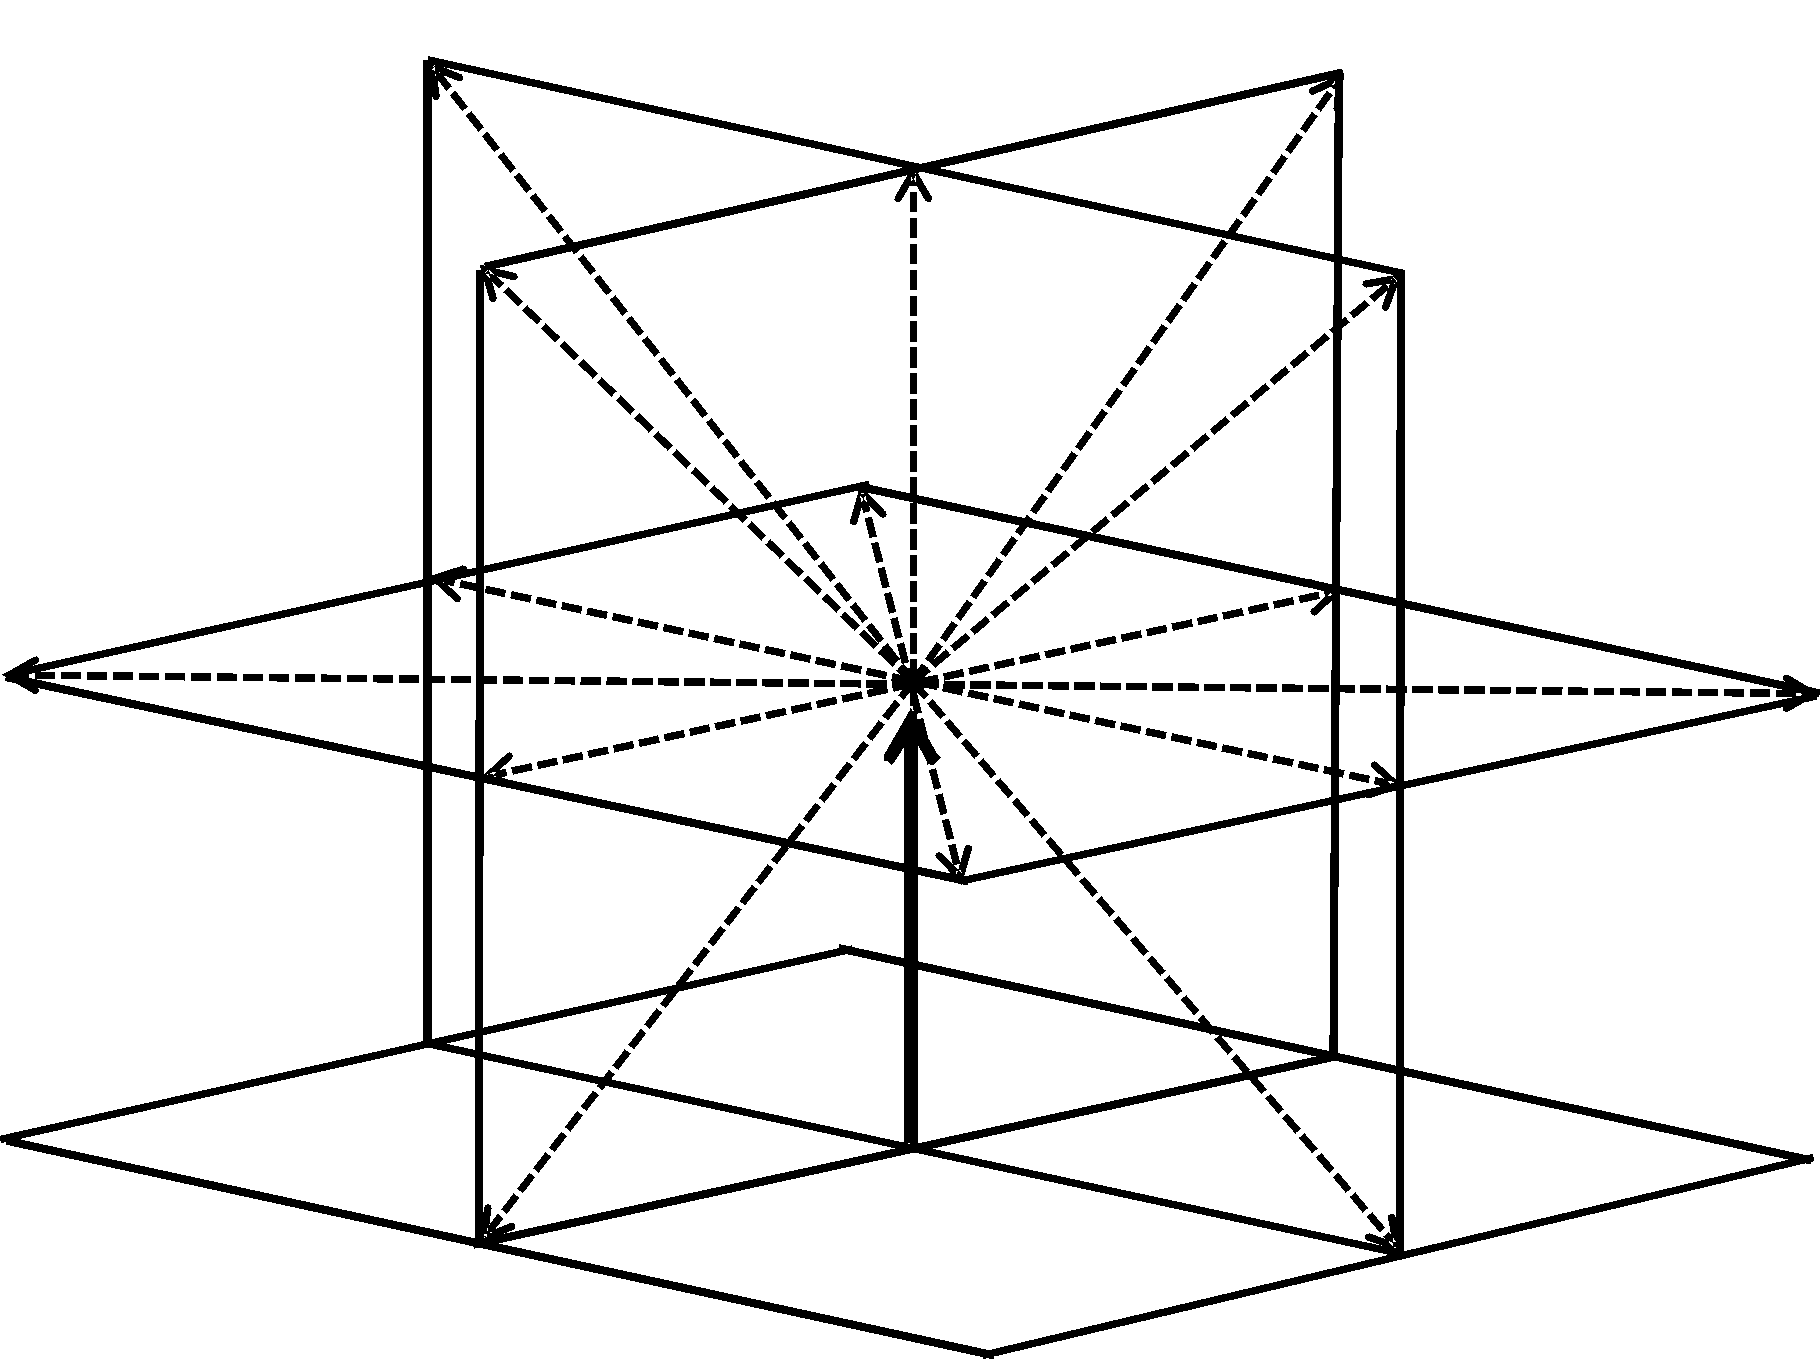
\includegraphics[width=0.9\textwidth]{imagens/5.png} 
			(a)\\
			\captionof{figure}{Esquema de desenvolvimento da árvore de descarga no espaço tridimensional: (a) as possíveis direções de desenvolvimento a partir do nó ativo; (b) o estado instantâneo do grafo de descarga. Os círculos correspondem aos nós do grafo condutor, e os números inscritos denotam os índices dos nós. O número de arestas direcionadas de entrada e saída (setas) para o nó dado é mostrado entre parênteses.}
		\end{minipage}
		\hfill
		\begin{minipage}{0.5\textwidth}
			\centering
			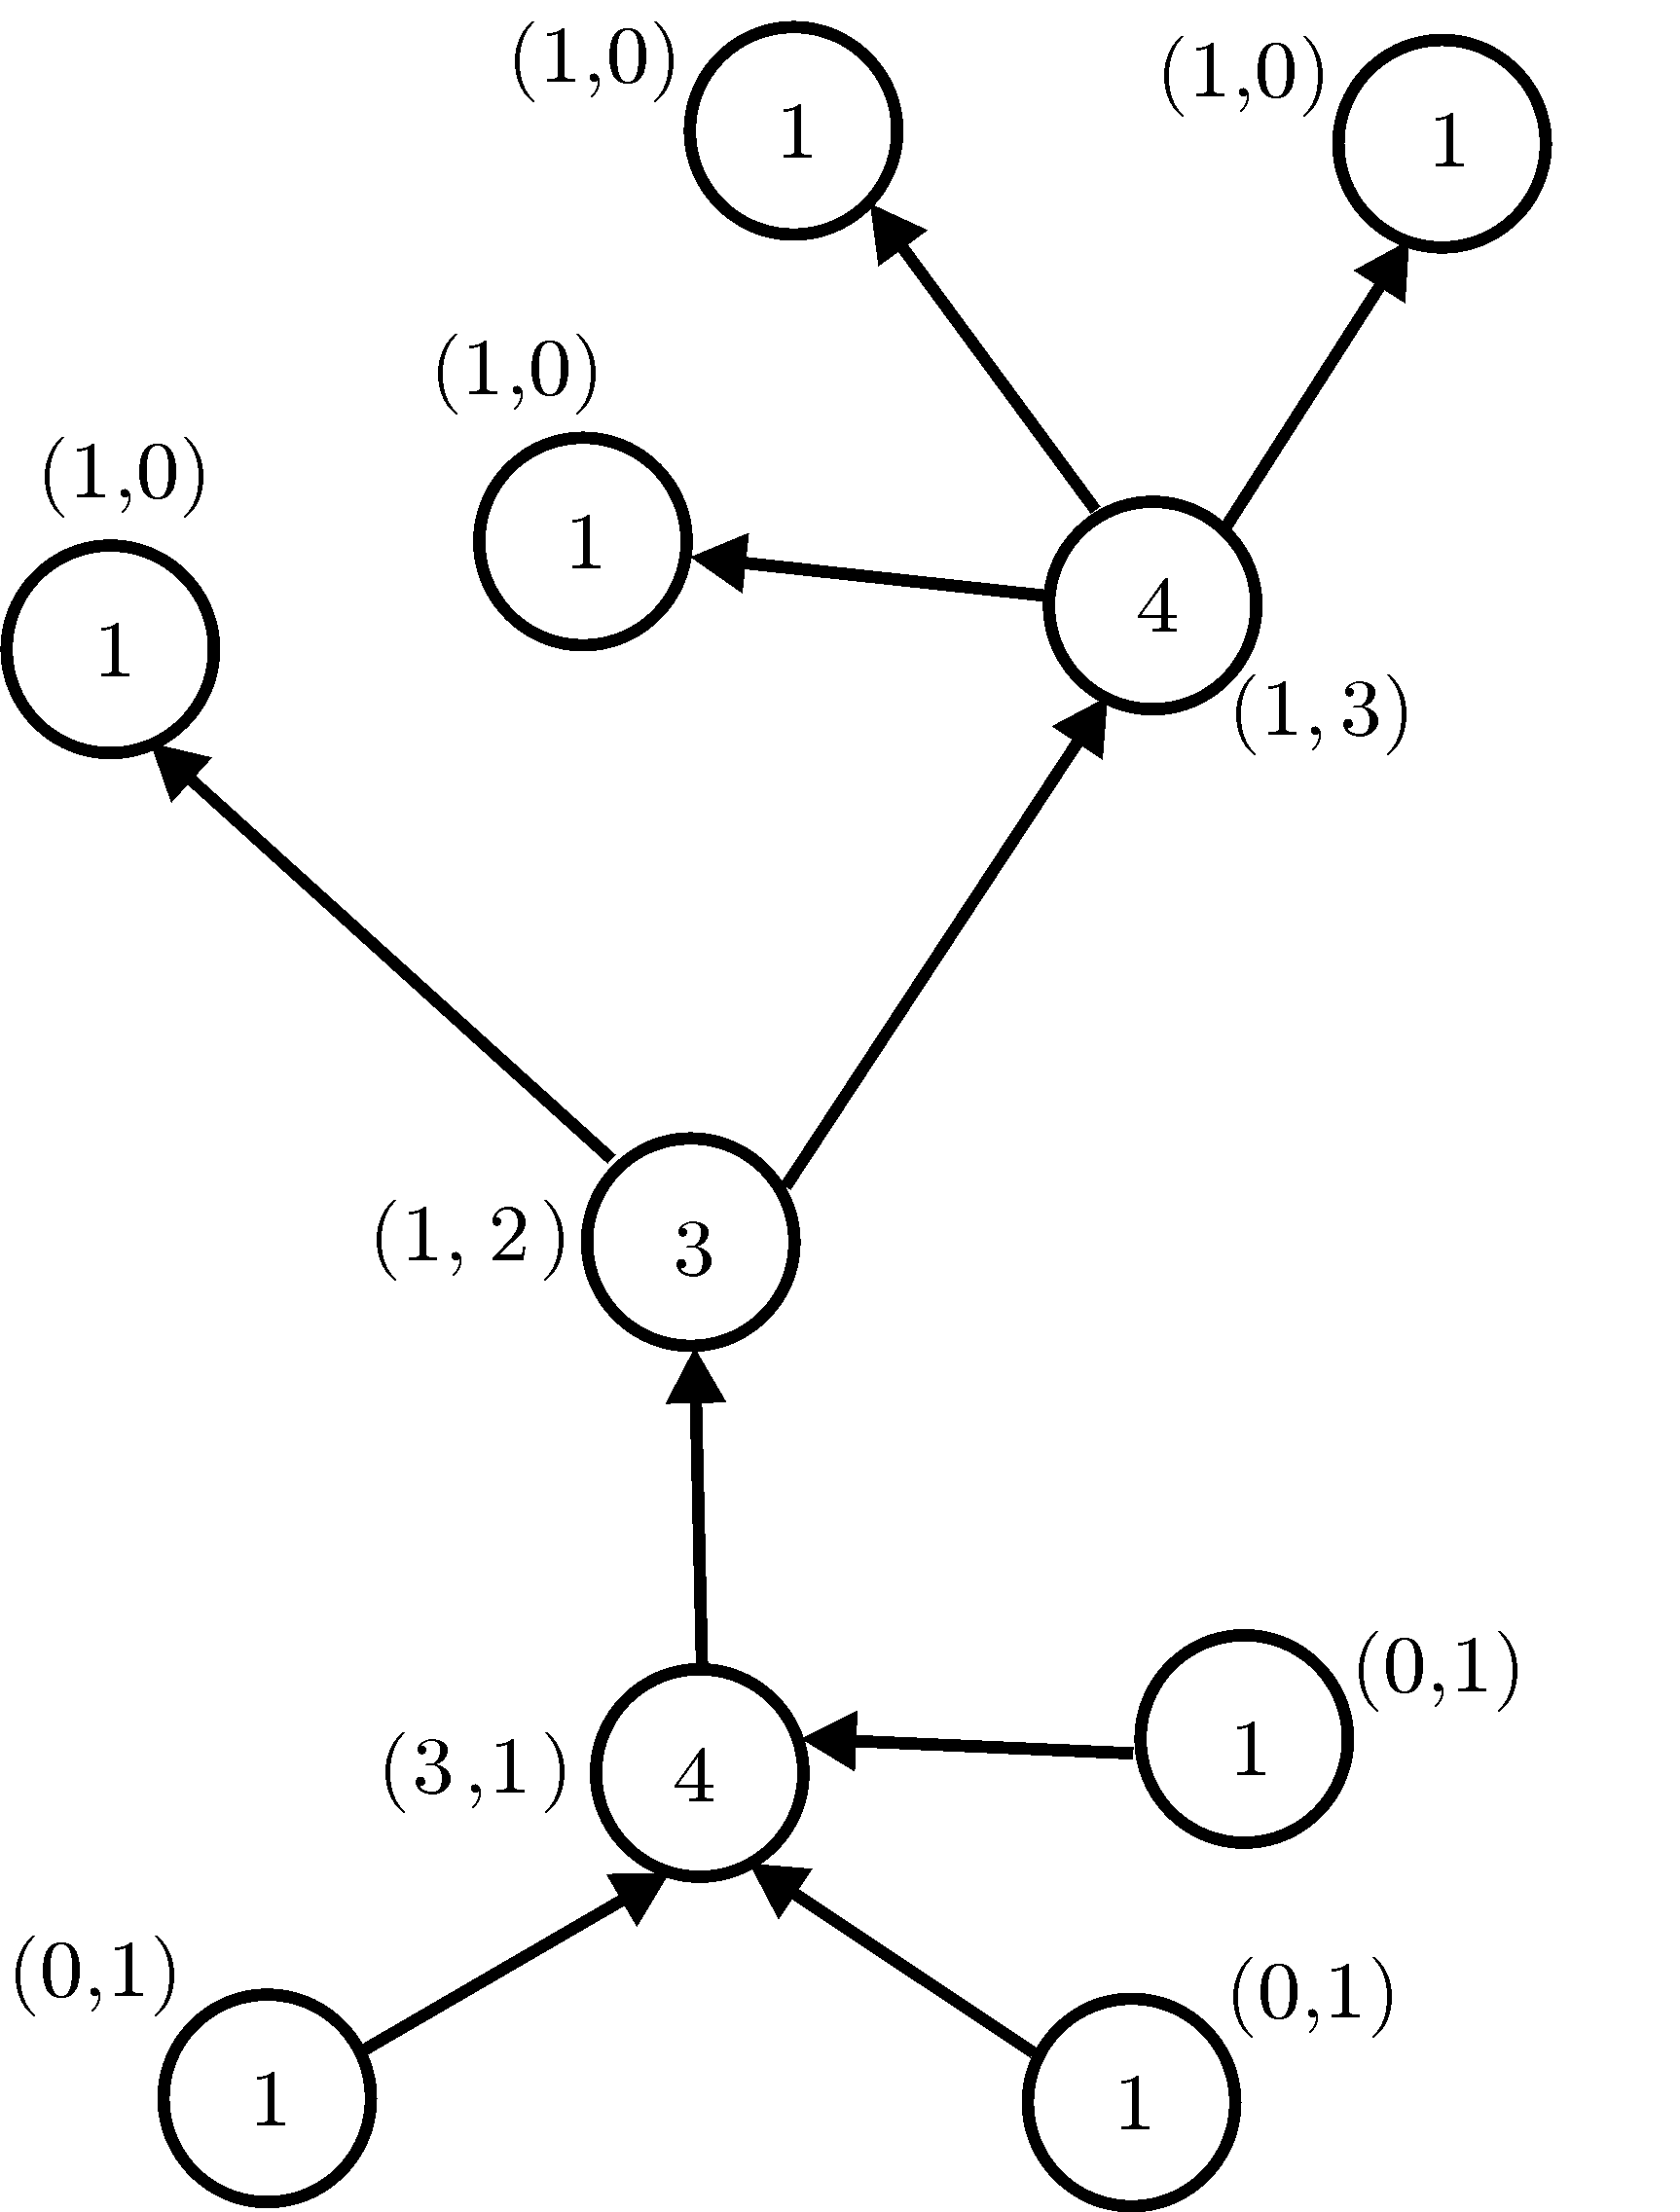
\includegraphics[width=\textwidth]{imagens/6.png} 
			(b)
		\end{minipage}
		 \label{fig:componente_m}
	\end{figure}

	O início da descarga ocorre espontaneamente para duas células vizinhas, em que a probabilidade de uma falha entre elas atinge o máximo. À medida que a descarga se desenvolve em diferentes partes da estrutura condutora gerada, novas conexões condutoras podem ser formadas, cuja probabilidade é descrita pela Equação~\ref{eqn_1}. A estrutura da descarga gerada é um grafo direcionado, cujos nós e arestas correspondem às células do domínio de simulação e ao acoplamento elétrico condutor. Todos os nós do grafo (árvore de descarga) podem ser divididos em três grupos não interseccionais: 1) nós periféricos que formam a fronteira externa da árvore, 2) nós intermediários que conectam sucessivamente os elos adjacentes de ramos individuais e 3) conexões de ramos, ou pontos de ramificação, ou seja, nós que são comuns a três ou mais elos. Se a intensidade do campo elétrico entre o nó periférico e as células mais próximas exceder o campo de iniciação, então um ou vários novos elos condutores, e o mesmo número de novos nós periféricos, surgem com a probabilidade (1). Se o nó periférico não ativar os elos com as células vizinhas, então ele morre junto com o elo condutor correspondente a ele.
	
	Para descrever a estrutura condutora, é conveniente introduzir a noção do índice do nó, que é igual ao número total de arestas direcionadas de entrada e saída (mostradas por setas na Figura 1; a direção das setas corresponde à direção da corrente). Por exemplo, o índice de um nó periférico é igual a um, o índice de um nó intermediário é igual a dois, etc. Cada um dos nós $i$ será colocado em correspondência com um par de números ($a_i$, $b_i$), que são iguais ao número de arestas de entrada e saída, respectivamente. A quantidade $a_i + b_i$ coincide obviamente com o índice do nó. A iniciação da carga corresponde à ocorrência de um par de nós adjacentes, onde um deles pertence ao tipo ($1, 0)$ e o outro ao tipo $(0, 1)$. No próximo passo do tempo do modelo, o estado do nó periférico ativo do tipo $(1, 0)$ se converte no estado $(1, n)$, onde n é o número de vizinhos recém-ativados do nó considerado. Da mesma forma, o estado do nó periférico ativo do tipo $(0, 1)$ se converte no estado $(n, 1)$. Dessa forma, todo o conjunto de nós da estrutura em evolução é distribuído entre os tipos $(1, n)$ e $(n, 1)$ com $n$ inteiro não negativo. O tronco da árvore de descarga é o núcleo não ramificado da estrutura, que é uma cadeia orientada composta por nós do tipo $(1, 1)$ e as arestas que os conectam. O tronco termina com um par de nós, onde um deles pertence ao tipo $(1, n)$ e o outro ao tipo $(n, 1)$. Os nós do tipo $(1, n)$ com $n \ge 2$ e as arestas de conexão formam a coroa, enquanto os nós do tipo $(n, 1)$ e as arestas de conexão formam a raiz da árvore orientada (veja Figura 1b).
	
	Uma característica importante do modelo considerado é a presença de um sistema de corrente que se desenvolve na estrutura condutora do \textit{streamer}. Isso torna o modelo discutido fundamentalmente diferente dos modelos fractais anteriores baseados na suposição de uma árvore de descarga exponencial em cada etapa do tempo do modelo. Nos canais condutores da árvore de descarga, há uma corrente elétrica que, por um lado, iguala os potenciais nos nós do grafo condutor e, por outro lado, satisfaz a lei da continuidade. Em cada etapa do tempo do modelo, a variação da carga elétrica na $i$-ésima célula elementar é dada pela relação.
	
	\begin{equation}
		dq_i = \tau \sum_{j=1}^{a_i + b_i} I_{ij} 
		\label{eqn_2}
	\end{equation}

	onde $I_{ij}$ é a corrente elétrica entre o $i$-ésimo e o $j$-ésimo nós com ligação condutora, que é determinada pela diferença de potenciais entre os nós $\phi_i - \phi_j$, a resistência linear de ligação $\Re_{ij}$ e seu comprimento $L_{ij}$, que, dependendo da orientação, pode assumir os valores $a$ ou $\sqrt{2}a$:
	\begin{equation}
		I_{ij} = \frac{\phi_i - \phi_j}{\Re_{ij} L_{ij}}
		\label{eqn_3}
	\end{equation}
	
	O potencial elétrico da i-ésima célula em cada etapa do tempo do modelo é determinado pela sua própria carga qi e pela capacitância efetiva, que para simplificação é assumida como igual à capacitância de uma esfera condutora de raio $a/2$, assim como o potencial total do campo elétrico, que é externo em relação ao domínio de simulação, e outras células carregadas do sistema. A variação da resistência linear é determinada pelo equilíbrio entre a liberação e a propagação do calor de Joule no canal de descarga. Uma vez que não existe uma descrição detalhada da dependência da resistência do canal de \textit{streamer} na corrente, assumimos que quando um canal surge, sua resistência linear é igual a $\Re_{0} = 0.1 M\Omega/m$, e à medida que a corrente aumenta no canal, seu valor diminui para $1 \mu \Omega/m$ para correntes maiores que $1 A$. Supõe-se que, à medida que a corrente varia no canal, um novo valor de resistência linear seja imediatamente estabelecido. O sistema resultante de canais condutores desempenha o papel de um sistema de drenagem da carga elétrica. Devido à soma das correntes dos canais individuais nos pontos de ramificação, a corrente no tronco de uma árvore de descarga excede significativamente as correntes em sua periferia. Observe que ao se mover dos elementos periféricos para o tronco, não apenas a intensidade da corrente aumenta, mas também o tempo de existência da ligação.
	
	A Figura \ref{fig:desenvolvimento_streamer} mostra um exemplo do desenvolvimento de uma única descarga de \textit{streamer} nas proximidades do campo elétrico máximo correspondente à fronteira entre as principais camadas de blindagem positiva e negativa da carga espacial (os parâmetros básicos da distribuição do campo foram discutidos anteriormente). É possível observar claramente que, com o desenvolvimento da descarga, o perfil do potencial entre sua coroa e raiz se torna mais plano; consequentemente, o campo elétrico dentro da descarga diminui. As regiões de máxima densidade de carga dentro da descarga estão concentradas na coroa e na raiz da descarga a alguma distância das extremidades periféricas, o que se deve à condutividade finita dos canais de \textit{streamer}. Assim, uma única descarga de \textit{streamer} bipolar, à medida que se desenvolve, é capaz de acumular uma carga elétrica significativa e, na verdade, forma um dipolo dinâmico distribuído, que desempenha um papel importante no desenvolvimento do \textit{CID}. Note que, em comparação com a duração da etapa principal do \textit{CID}, a carga em uma única descarga de \textit{streamer} bipolar é acumulada lentamente (por até algumas dezenas de milissegundos). As correntes no tronco da descarga não excedem alguns amperes, o que implica que sua radiação eletromagnética é relativamente fraca.
	
	\begin{figure}[!h]
		\centering
		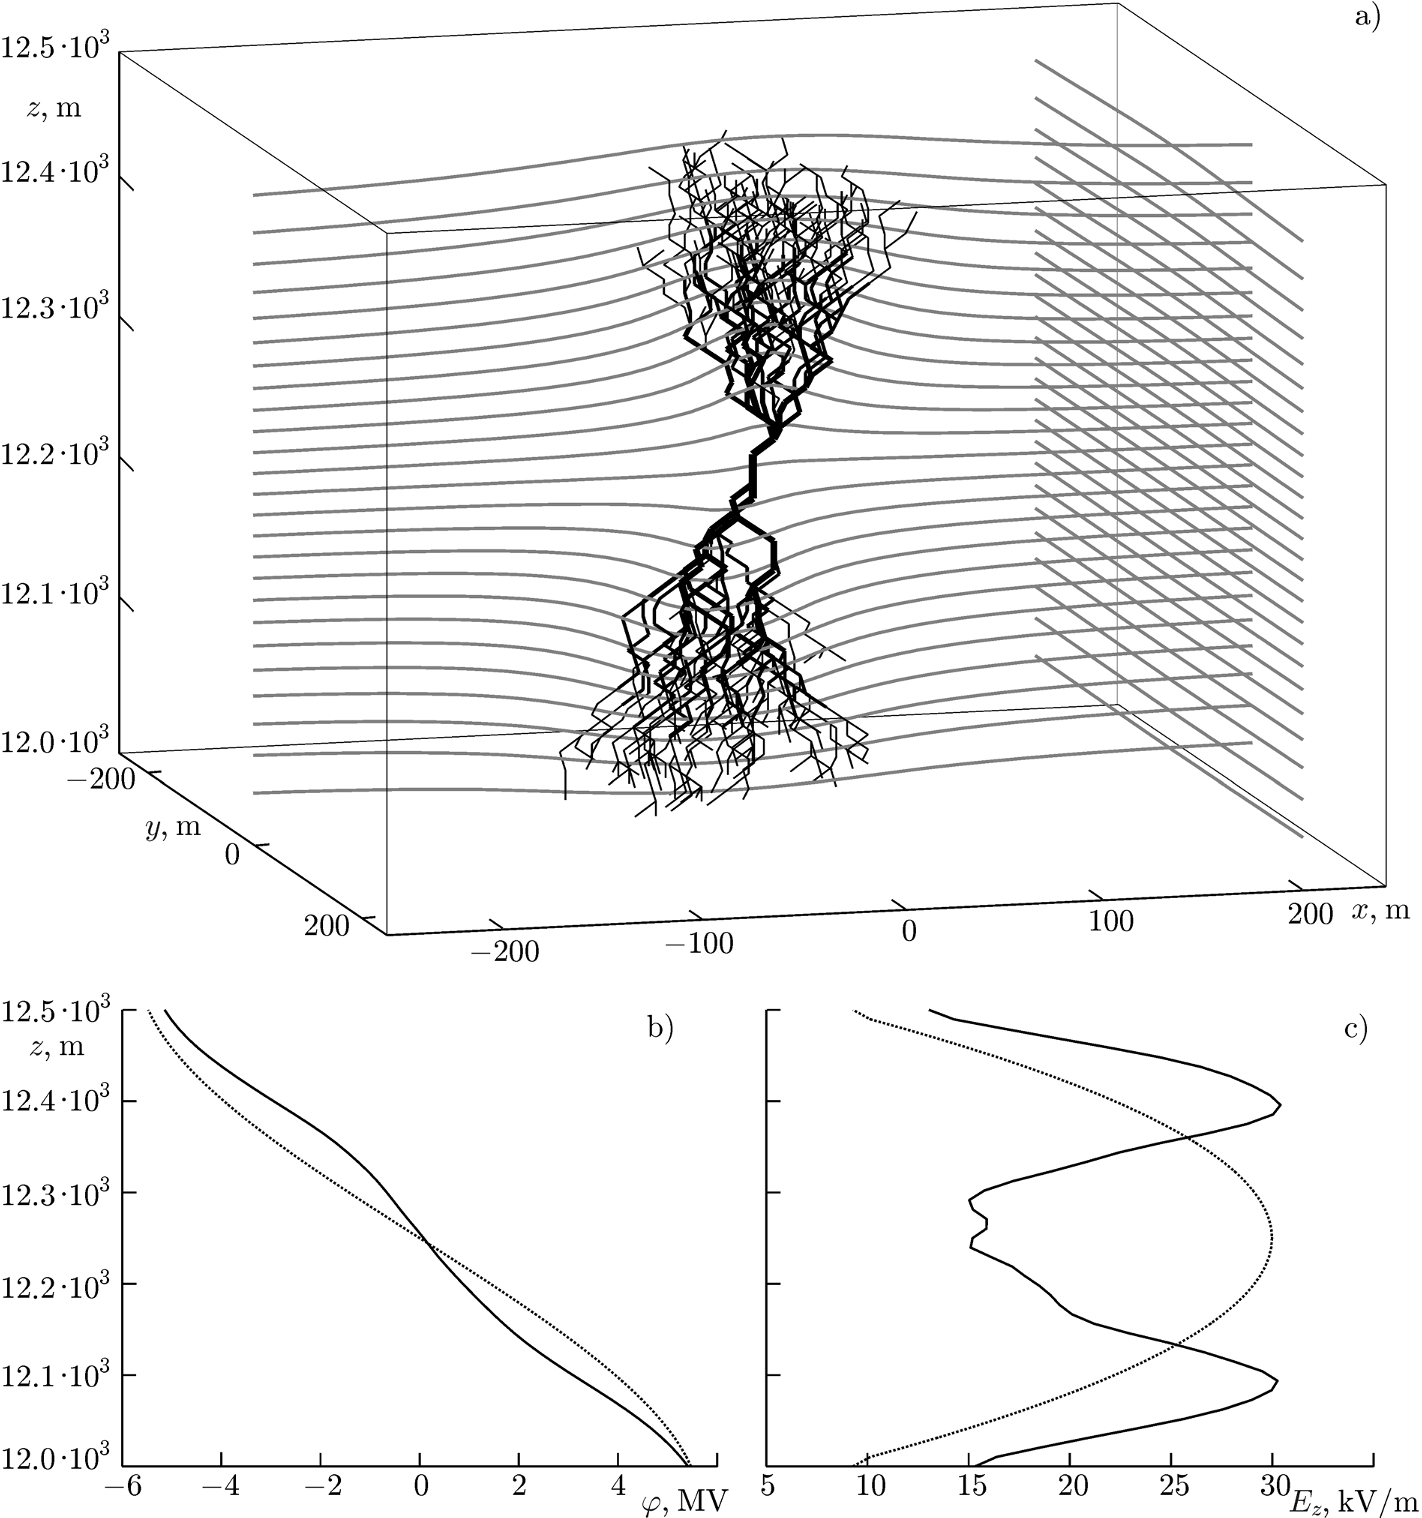
\includegraphics[width=0.9\textwidth]{imagens/9.png}
		\caption{(a) Uma imagem instantânea de uma descarga de streamer bipolar tridimensional em um canal elétrico fracamente não uniforme. A espessura do elemento do gráfico corresponde à intensidade da corrente no canal condutor correspondente. As linhas cinzas correspondem aos equipotenciais nos planos $y = 0$ e $x = 200 m$; doravante, $x$ e $y$ são os eixos do sistema de coordenadas cartesianas, e $r \bot (x, y)$. Perfis de altitude do potencial elétrico (b) e do componente vertical do campo elétrico (c) antes da geração do canal (linha tracejada) e no estágio de uma descarga desenvolvida (linha contínua).}
		\label{fig:desenvolvimento_streamer}
	\end{figure}
	
	\subsection{A SINCRONIZAÇÃO DA DESCARGA DE STREAMER E A INICIAÇÃO DO \textit{CID}}
	
	Conforme mencionado anteriormente, o modelo considerado para a iniciação do \textit{CID} pressupõe a formação de duas estruturas de \textit{streamer} bipolar desenvolvidas que acumularam uma carga elétrica significativa antes do momento da interação. Nesse caso, a sincronização espaço-temporal das descargas de \textit{streamer} é importante: elas devem se desenvolver ao mesmo tempo a uma distância relativamente curta uma da outra ao longo do campo elétrico externo. É observado na Figura \ref{fig:desenvolvimento_streamer}b que, em princípio, à medida que uma única descarga se desenvolve, o campo elétrico em seu eixo é reforçado na fronteira da descarga. Devido a isso, o campo no eixo da descarga, especialmente na presença de uma pequena inomogeneidade aleatória de densidade de carga, pode exceder em algum momento o limite de iniciação, resultando em mais uma descarga de \textit{streamer}. No entanto, esse método de sincronização das descargas possui uma desvantagem significativa: a distância entre as duas descargas é muito pequena para o desenvolvimento independente delas e para a coleta de uma carga espacial suficiente antes do contato elétrico. Como resultado, o campo no espaço entre as descargas atinge rapidamente um valor de ruptura, e a segunda descarga se torna parte da primeira descarga mais desenvolvida sem a iniciação do \textit{CID}. Geralmente, na presença de variações na densidade de carga com uma escala característica da ordem do tamanho longitudinal (ao longo do campo elétrico externo) da estrutura de \textit{streamer} bipolar, o campo pode exceder o valor de limite e iniciar a segunda descarga a distâncias muito maiores da primeira descarga. Como resultado, antes do contato com a primeira descarga de \textit{streamer}, a segunda descarga tem tempo para acumular uma carga elétrica suficiente para a iniciação do \textit{CID}.
	
	A fonte de variações de grande escala na densidade de carga e, consequentemente, no campo elétrico pode ser a componente turbulenta do fluxo convectivo, que é intensificada na borda superior da nuvem. No entanto, devido às diferentes escalas das perturbações na densidade de carga, pode-se esperar uma ampla dispersão dos parâmetros do \textit{CID}, o que, no entanto, é pouco confirmado pelas observações. Nesse sentido, é interessante estudar os mecanismos capazes de formar uma perturbação de grande escala quase regular no campo elétrico (densidade de carga), em relação à qual as descargas de \textit{streamer} podem se desenvolver na etapa preliminar do \textit{CID}. Um possível mecanismo para a formação da distribuição inomogênea da densidade de carga com a escala espacial necessária pode ser a instabilidade do fluxo, que foi descrita pela primeira vez em [54]. Essa instabilidade se desenvolve em um meio interno multicomponente em presença de um fluxo de ar fracamente condutor em relação às partículas mais pesadas presentes na nuvem. Como resultado, uma onda de carga espacial com crescimento exponencial é formada na nuvem; ela se desloca com o fluxo convectivo em direção ao topo da nuvem. A taxa de crescimento da densidade de carga no referencial do fluxo,
	
	\begin{equation}
		\gamma_{max} = \begin{cases}
							4\pi\sigma\left(\Omega/\vartheta-1\right)^2, & \Omega/\vartheta < 2 \\ 
							2\pi\sigma/\vartheta, & \Omega/\vartheta > 2 
					   \end{cases}
		\label{eqn_4}	
	\end{equation}

	é determinada pelo análogo da frequência do plasma para partículas pesadas,$\Omega^2 = 4\pi Q^2N/M$ onde $Q$, $M$ e $N$ são a carga, massa e densidade das partículas pesadas, respectivamente, a frequência efetiva $\vartheta$ de suas colisões e a condutividade do fluxo de ar $\sigma$. Nesse caso, a escala espacial $2 pi /k_{opt}$ da inomogeneidade gerada na densidade de carga também depende da velocidade do fluxo de ar $u$:
	
	\begin{equation}
		k_{opt} = \begin{cases}
						\frac{\vartheta}{u} \left(\frac{\Omega}{\vartheta}-1\right)^{\frac{1}{2}}& \Omega/\vartheta < 2 \\ 
						\sigma/\vartheta, & \Omega/\vartheta > 2 
				  \end{cases}
				  \label{eqn_5}	
	\end{equation}

	De acordo com as estimativas [54], o tempo característico de desenvolvimento da instabilidade é da ordem de 100 segundos e a escala espacial da inomogeneidade da carga pode variar amplamente de dezenas a centenas de metros. Devido ao pequeno tamanho da região considerada, o efeito das condições de contorno na distribuição da densidade de carga pode ser negligenciado. Uma análise mais detalhada da instabilidade do fluxo com consideração dos mecanismos de carga e dos parâmetros das partículas da nuvem é apresentada em [55]. Apenas observamos que o mencionado mecanismo de formação de não uniformidade do campo elétrico é bastante robusto em relação às características das partículas pesadas e à intensidade do campo elétrico externo. A presença de partículas relativamente pesadas nas camadas superiores da nuvem pode ser atribuída a um aumento de curta duração dos fluxos ascendentes na nuvem de tempestade. O fato de os fluxos convectivos locais terem um efeito significativo no início do \textit{CID} é favorecido pelo agrupamento espaço-temporal observado de descargas compactas, que se manifesta como um aumento abrupto na taxa de ocorrência delas em uma região limitada da nuvem, na fronteira das camadas carregadas. De acordo com [23], a taxa de ocorrência de \textit{CIDs} negativos, que são mais raros em geral, pode superar por algum tempo a taxa de ocorrência de \textit{CIDs} positivos. Isso pode estar relacionado à formação de condições favoráveis para o desenvolvimento sincronizado de descargas de fluxo devido à instabilidade do fluxo.
	
	O desenvolvimento do \textit{CID} em um meio com distribuição não uniforme do campo elétrico e carga espacial é ilustrado na Figura 3, onde a distribuição inicial em larga escala da densidade de carga na região de iniciação do CID, que corresponde ao perfil do campo elétrico na Figura \ref{fig:desenvolvimento_streamer}c, é complementada com uma perturbação harmônica com uma escala espacial de 200 m (curvas 1 na Figura 3). Observa-se que, com o desenvolvimento da primeira descarga que ocorreu a uma altitude de cerca de 12350 $m$, o campo elétrico nela aumenta. Acima e abaixo da primeira descarga, nas altitudes correspondentes ao meio período da perturbação do campo de polaridade negativa, o campo total permanece muito menor do que o campo de iniciação da descarga de fluxo. Como resultado, uma espécie de banda proibida para a iniciação da segunda descarga é formada nas imediações da primeira descarga. Por outro lado, nos meio períodos vizinhos da perturbação positiva do campo, à medida que a primeira descarga se desenvolve, as condições para a iniciação da segunda descarga tornam-se cada vez mais favoráveis (em particular, um leve aumento do máximo local do campo a uma altitude de cerca de 12140 $m$ é observado na Figura 3c). Como resultado, em um meio com a considerada distribuição quasiperiódica da densidade de carga, o desenvolvimento de uma descarga de fluxo bipolar leva necessariamente à iniciação da segunda descarga de fluxo, que é separada da primeira descarga pela região de baixo campo elétrico. O atraso da segunda descarga é pequeno em comparação com a duração da etapa preliminar do \textit{CID} e não leva a uma diferença significativa das descargas de fluxo no momento do contato elétrico. Observa-se que durante a formação de vários períodos da inomogeneidade espacial da densidade de carga, há a possibilidade da iniciação sucessiva de vários \textit{CIDs}.
	\begin{figure}
		\label{fig:desenvolvimento_CID}
		\begin{minipage}{0.5\textwidth}
			\centering
			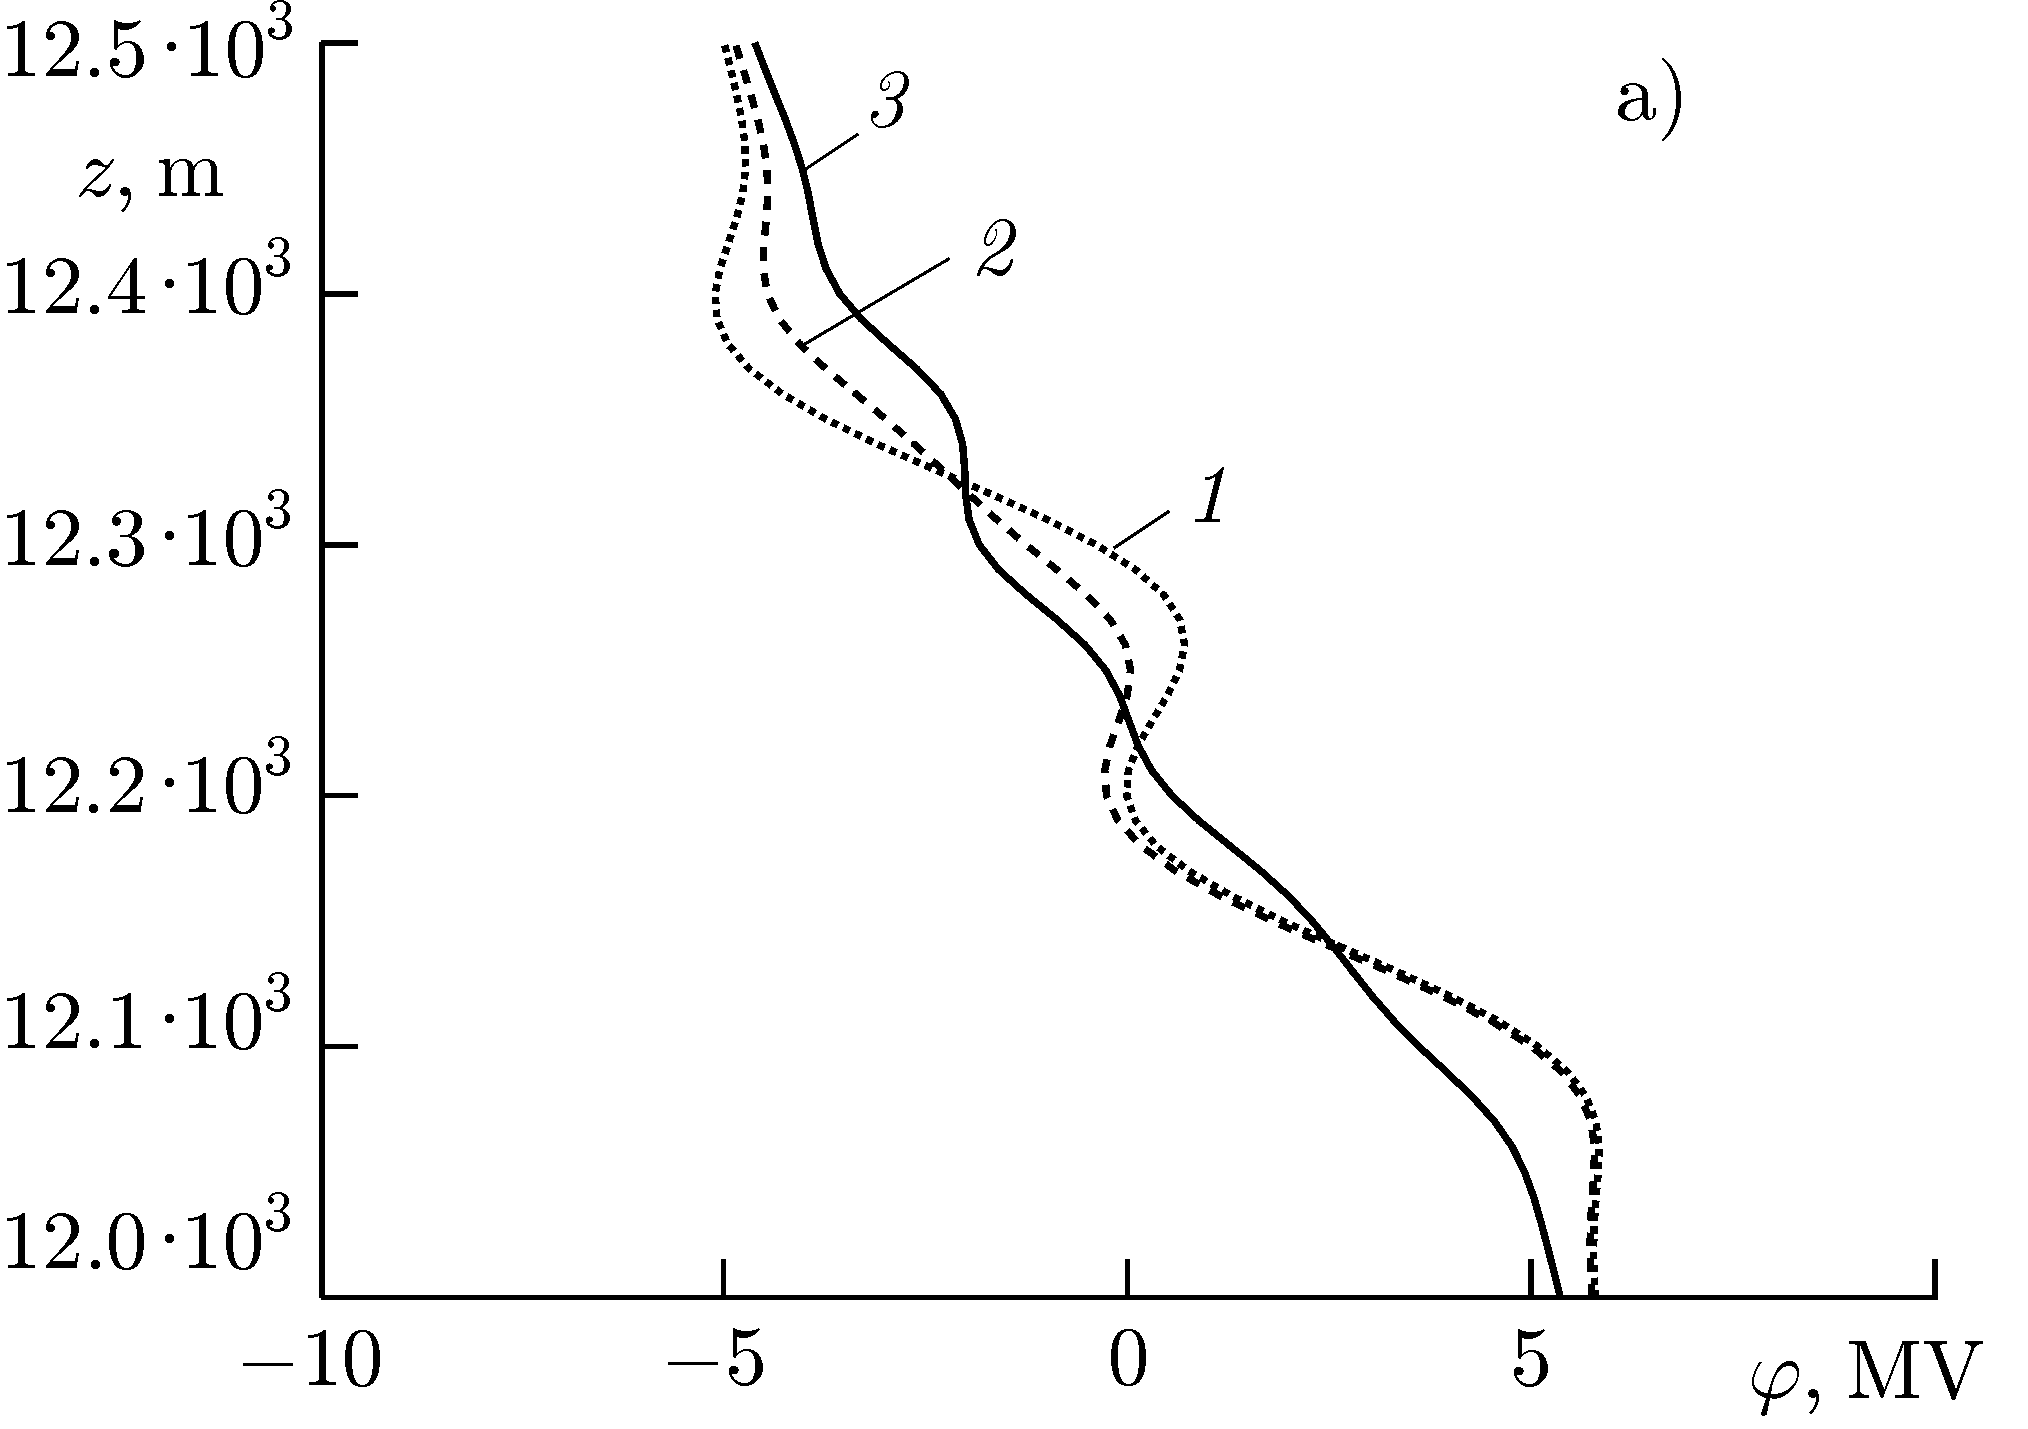
\includegraphics[width=0.95\textwidth]{imagens/12a.png}
			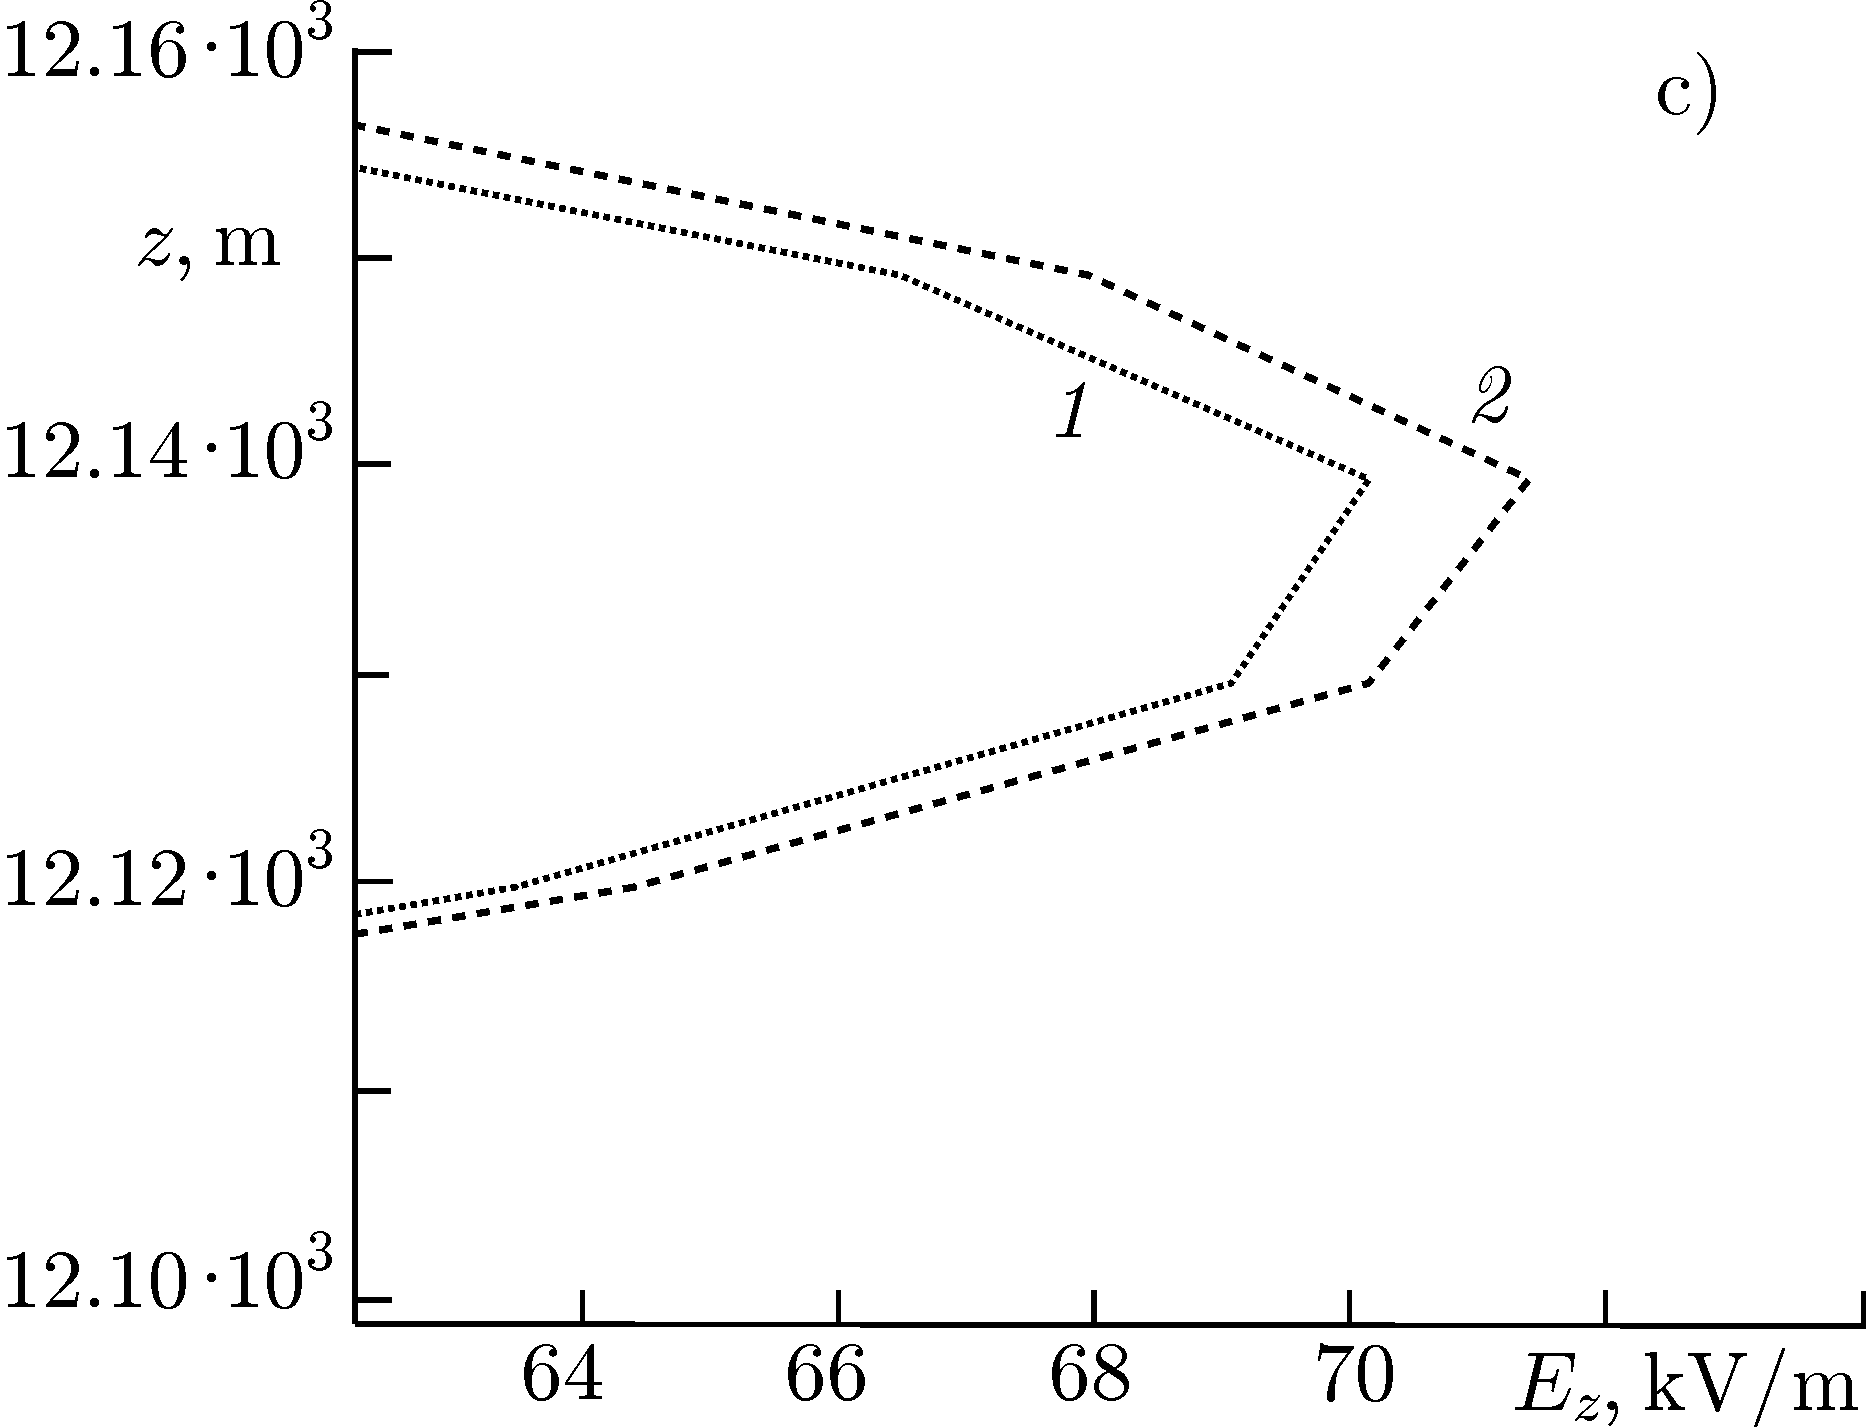
\includegraphics[width=0.95\textwidth]{imagens/13.png}
		\end{minipage}
		\begin{minipage}{0.5\textwidth}
			\centering
			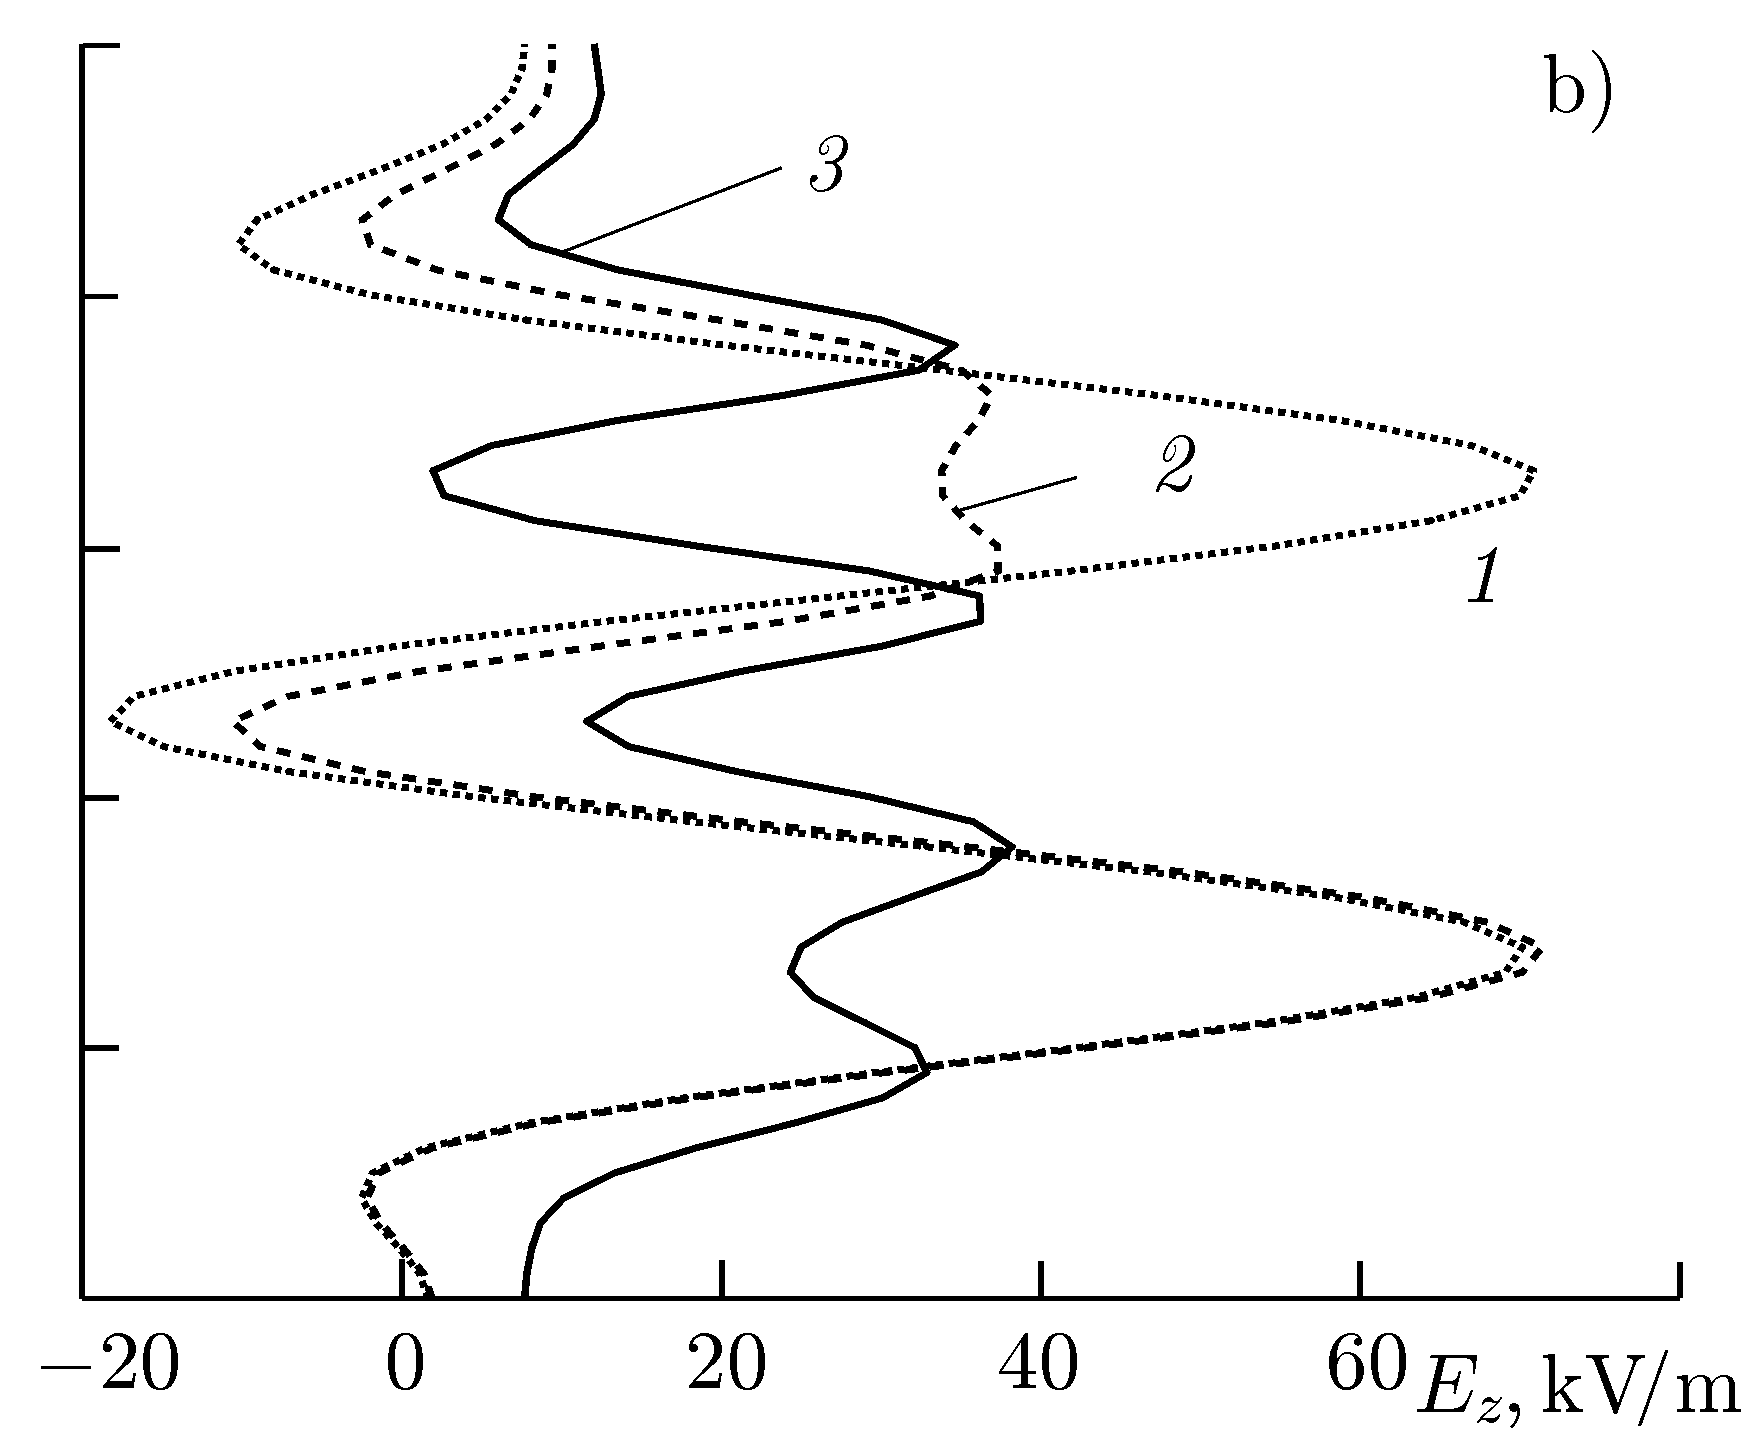
\includegraphics[width=0.95\textwidth]{imagens/12b.png}
			\captionof{figure}{Perfis de altitude do potencial (a) e componente vertical do campo elétrico (b e c) em diferentes momentos da etapa preliminar do \textit{CID}. As curvas 1 correspondem ao momento da ocorrência da primeira descarga, as curvas 2 correspondem ao momento da ocorrência da segunda descarga e as curvas 3 correspondem ao momento do contato elétrico das descargas e formação do canal de corrente do \textit{CID}. As curvas são plotadas ao longo da linha que passa pelo ponto de iniciação da descarga.}
		\end{minipage}
	\end{figure}
	
	A Figura 4 mostra instantâneos de diferentes estágios da evolução do CID em um meio com um campo elétrico espacialmente não uniforme, cuja distribuição no eixo da região de cálculo é semelhante ao perfil apresentado na Figura 3. Observa-se que a segunda descarga surge com um atraso de aproximadamente 5 $ms$ após a iniciação da primeira descarga (ver Figuras 4a e 4b), e depois disso, ambas as descargas existem simultaneamente por um longo período (ver Figura 4c). Como resultado da redistribuição de carga por cada uma das descargas de fluxo, a queda de campo elétrico entre as descargas diminui até que ocorra um contato elétrico entre as estruturas de descargas de fluxo cerca de 11 $ms$ após a iniciação da segunda descarga (ver Figura 4d).
	
	\begin{figure}[!h]
		\centering
		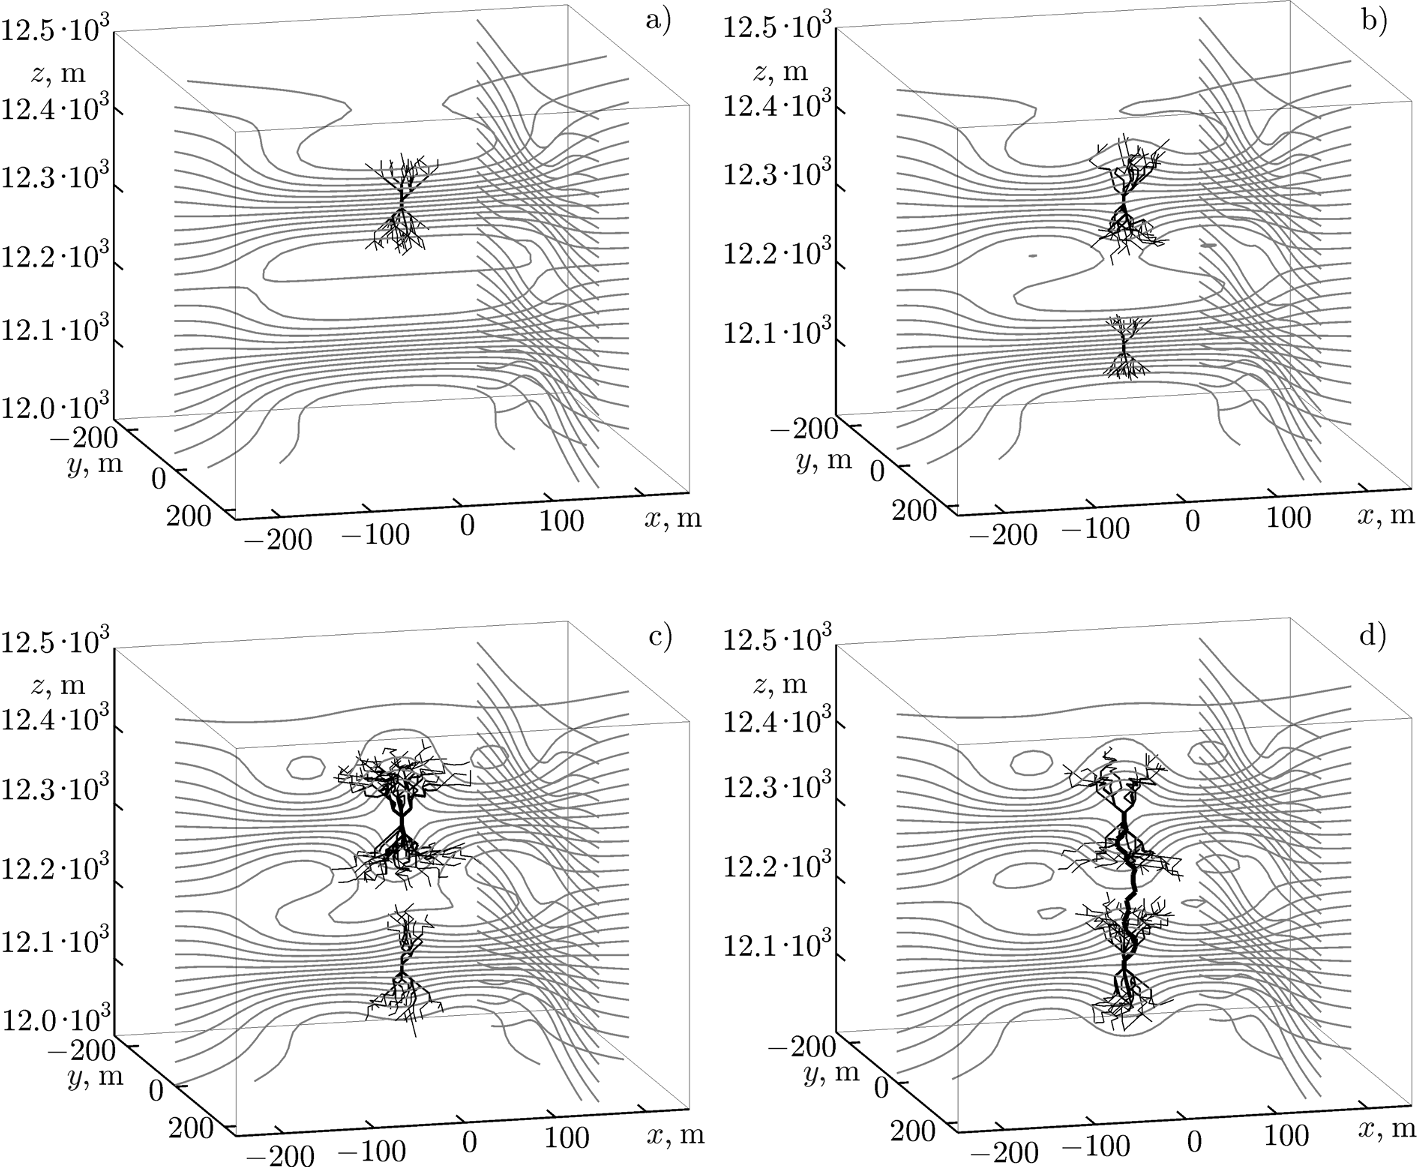
\includegraphics[width=0.9\textwidth]{imagens/14.png}
		\caption{Estágios sucessivos do desenvolvimento do \textit{CID} em um meio com campo magnético externo espacialmente não uniforme: (a) o desenvolvimento da primeira descarga de \textit{streamer} em sete etapas do tempo do modelo ($t = 140 \mu s$); (b) o início do desenvolvimento da segunda descarga ($t = 5,06 ms$); (c) o desenvolvimento simultâneo do par de descargas ($t = 7,50 ms$); (d) o instante do contato elétrico das descargas após 556 etapas do tempo do modelo ($t = 11,12 ms$) com a formação de um canal de alta corrente. As linhas cinzas correspondem às equipotenciais nos planos $y = 0$ e $x = 200$ $m$.}
		\label{fig:desenvolvimento_passo_a_passo_CID}
	\end{figure}
	
	A descrição da etapa principal do \textit{CID}, na qual um canal de corrente de alta potência é formado entre as descargas de \textit{streamer}, está intimamente relacionada com a emissão de radiação de baixa e alta frequência do \textit{CID}. As características da radiação das descargas compactas são consideradas com mais detalhes na segunda parte do trabalho. Aqui, fornecemos apenas algumas das características do surgimento de uma rajada de corrente. Como mencionado anteriormente, um requisito para a formação de um pulso curto de corrente de alta potência no \textit{CID} é a presença de regiões relativamente próximas de carga espacial com sinal oposto, que são formadas na etapa preliminar de uma descarga. A estrutura de tais regiões é ilustrada na Figura 5, que mostra a distribuição inicial da densidade de carga na nuvem e uma distribuição semelhante antes da quebra, no início da etapa principal do \textit{CID}. É possível observar que, nesse instante, a carga volumétrica nas regiões adjacentes das descargas de \textit{streamer} bipolares está compactamente concentrada nas proximidades do canal de quebra, sendo a densidade de carga antes da quebra quase vinte vezes maior do que o valor inicial.
	
	\begin{figure}[!h]
		\label{fig:distribuicao_de_cargas}
		\begin{minipage}{0.48\textwidth}
			\centering
			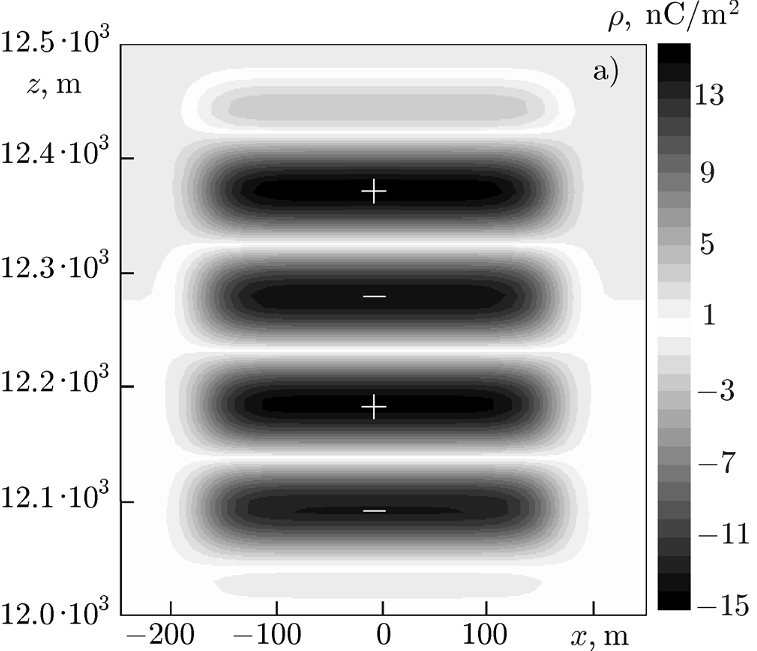
\includegraphics[width=\textwidth]{imagens/15a.png}
			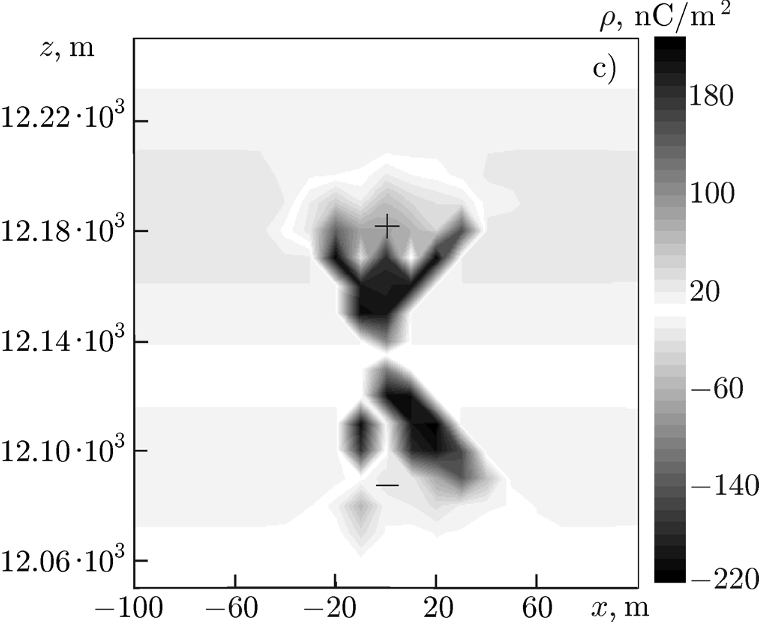
\includegraphics[width=\textwidth]{imagens/16.png}
		\end{minipage}
		\begin{minipage}{0.48\textwidth}
			\centering
			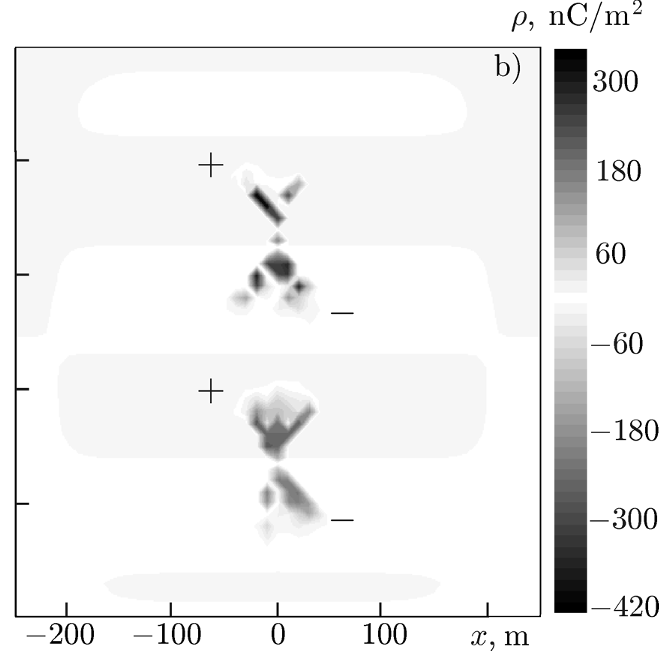
\includegraphics[width=\textwidth]{imagens/15b.png}
			\captionof{figure}{Distribuição espacial da densidade de carga elétrica (a) antes do momento de iniciação da primeira descarga de \textit{streamer} e (b e c) no momento do início da etapa principal do \textit{CID}, quando o canal com corrente forte é formado. Observa-se que, no momento do início da etapa principal do \textit{CID}, a densidade de carga acumulada em cada estrutura de \textit{streamer} bipolar aumenta em mais de vinte vezes.}
		\end{minipage}
	\end{figure}

	A distribuição da densidade de carga ao longo do canal condutor entre as descargas de \textit{streamer} no momento de sua ocorrência é mostrada na Figura 6a, e a correspondente distribuição da corrente de descarga em diferentes momentos de tempo após o início da etapa principal do CID é apresentada na Figura 6b, assumindo que a velocidade da frente de onda de ionização é de $6 \times 10^7 m/s$. Observa-se que a amplitude da corrente de descarga é de aproximadamente 45 $kA$ com uma duração de cerca de $10 \mu s$, o que concorda bem com as estimativas dos parâmetros do pulso de corrente do \textit{CID}, que foram obtidas no âmbito da aproximação de linha de transmissão [27]. Dentro da descrição proposta, é possível considerar de forma natural várias características da corrente de descarga que não podem ser analisadas na aproximação de linha de transmissão. Em particular, neste modelo, é possível levar em conta a deformação da forma do canal em relação à linha reta, o possível ramificação do canal de corrente, diferenças na velocidade de propagação do pulso de corrente em diferentes direções, sua assimetria espaciotemporal, etc. Essas questões, juntamente com a verificação da suposição de um baixo nível de radiação eletromagnética na etapa preliminar do \textit{CID} e a formação de uma rajada curta de alta potência de radiação \textit{HF/VHF}, serão discutidas na segunda parte do trabalho. Para concluir, observamos que os resultados obtidos no âmbito da abordagem proposta, em particular, a forma e as características da estrutura de \textit{streamer} bipolar na etapa preliminar do \textit{CID}, são em grande parte determinados pelos parâmetros escolhidos dos elementos do modelo, como o tamanho e capacitância efetiva de uma célula elementar, taxa de formação do canal condutor entre as células e a dependência de sua condutividade da corrente que flui por ele. Como mencionado anteriormente, a complexidade e a diferença de escala dos processos durante as descargas elétricas na nuvem de tempestade levam necessariamente à sua parametrização. No entanto, muitas questões na física das descargas gasosas não têm respostas unívocas; portanto, a escolha de tal parametrização neste modelo é baseada em suposições comuns sobre a estrutura e as características de uma descarga. É óbvio que a construção de uma parametrização mais exata e justificada requer mais experimentos e estudos teóricos, principalmente, na microfísica das descargas nas nuvens de tempestade. Ao mesmo tempo, a abordagem proposta neste artigo também pode ser usada para determinar a faixa de parâmetros dos elementos do modelo em que o modelo descreve satisfatoriamente as características observadas das descargas compactas intra-nuvem.
	
	\begin{figure}[!h]
		\centering
		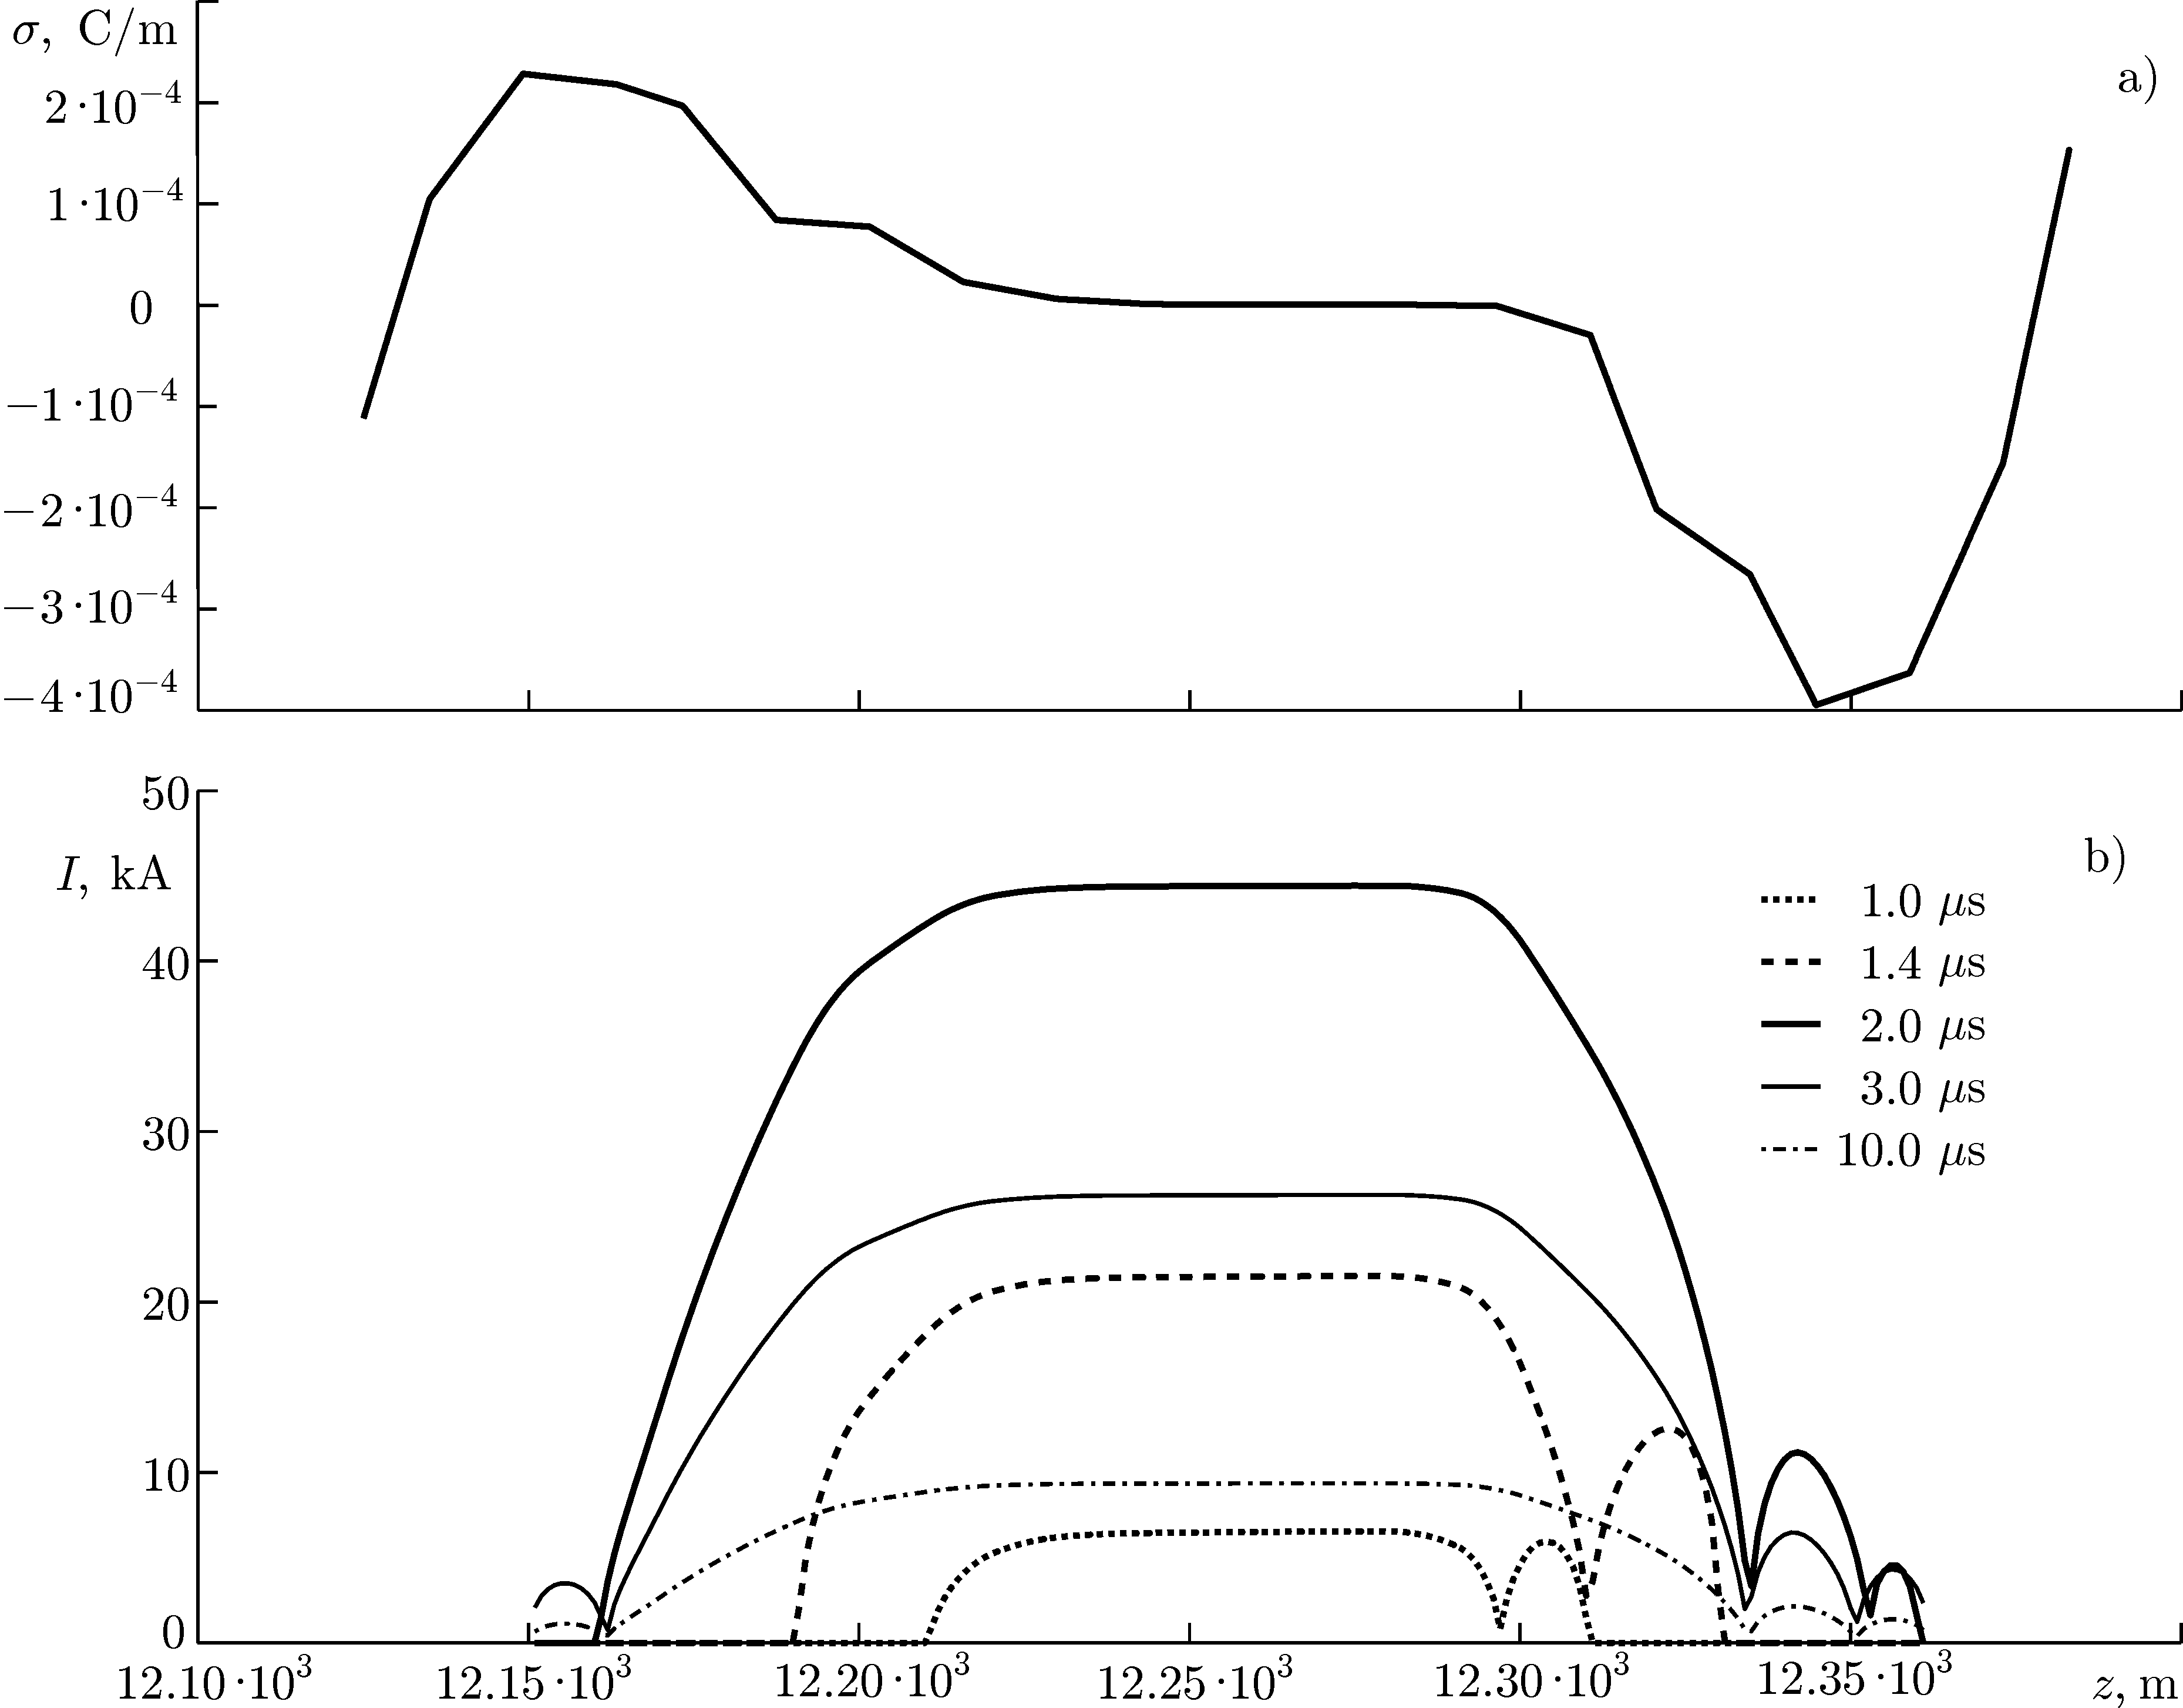
\includegraphics[width=0.8\textwidth]{imagens/17.png}
		\caption{	Distribuições da densidade linear $\sigma$ da carga elétrica ao longo do canal condutor, que conecta as estruturas de \textit{streamer} bipolar, no momento de sua ocorrência (a) e corrente elétrica $I$ nesse canal em diferentes momentos de tempo após o início da etapa principal do \textit{CID} (b). A distribuição de corrente ao longo do canal condutor foi obtida para o passo de tempo do modelo igual a $\tau = 0,2 \mu s$.}
	\end{figure}
	\pagebreak
	\section{CONCLUSÕES}
	
	Propusemos um novo modelo de uma descarga compacta intra-nuvem, que sugere que esta última é o resultado da interação de duas (ou mais) estruturas de \textit{streamer} bipolar que se formam em um campo elétrico de grande escala. O modelo pressupõe que a \textit{CID} se desenvolve em duas etapas. Na etapa preliminar, duas ou mais estruturas de \textit{streamer} bipolar ocorrem sucessivamente no campo de um forte campo elétrico (por exemplo, na fronteira das principais camadas positivas e negativas de carga espacial ou na fronteira das principais camadas de blindagem positivas e negativas). Presumivelmente, a sincronização espaço-temporal das estruturas de \textit{streamer} é fornecida pela modulação em altitude do campo elétrico, e a instabilidade de corrente é uma possível fonte dessa modulação. É mostrado que durante o seu desenvolvimento, uma única estrutura de \textit{streamer} bipolar acumula uma carga elétrica significativa e é efetivamente um dipolo dinâmico distribuído. O início da etapa principal da \textit{CID} corresponde ao momento de um acoplamento elétrico entre as estruturas de streamer, no qual a carga elétrica acumulada nas extremidades adjacentes das descargas é neutralizada em um tempo muito mais curto do que a duração da etapa preliminar da \textit{CID}. Nesse caso, os parâmetros do pulso de corrente gerado concordam bem com as estimativas de corrente da \textit{CID} obtidas na aproximação da linha de transmissão. Dentro da abordagem proposta, parece possível explicar uma série de características observadas da \textit{CID}, em particular, a fraca radiação (abaixo dos limiares de detecção estabelecidos nos experimentos) na etapa preliminar de uma descarga, a formação de um curto pulso bipolar de campo elétrico de alta potência e a sincronização das explosões de radiação nas faixas \textit{VLF/LF} e \textit{HF/VHF}. A radiação de uma descarga compacta intra-nuvem em diferentes faixas de frequência será considerada na segunda parte do trabalho.
	
	Os autores agradecem a V. A. Rakov pela discussão frutífera dos resultados e pelos comentários importantes, assim como a N. A. Bogatov, A. Yu. Kostinsky e E. A. Mareev pelas discussões úteis. Este trabalho foi apoiado pela Fundação Russa de Pesquisa Básica (projetos Nos. 13-05-01100 e 15-01-06612) e pelo Ministério da Educação e Ciência da Federação Russa (contrato estatal No. 14.B25.31.0023).
	
	\begin{thebibliography}{99}
\bibitem{} D. M. Le Vine, J. Geophys. Res., 85, No. C7, 4091 (1980).
\bibitem{} J. C. Willett, J. C. Bailey, and E. P. Krider, J. Geophys. Res., 94, No. D13, 16255 (1989).
\bibitem{} P. J. Medelius, E. M. Thomson, and E. M. Pierce, in: Proc. Int. Aerospace and Ground Conf. Lightning	and Static Electr., NASA Conf. Publ., 1991, Vol. 3106, p. 12-1.
\bibitem{} D. N. Holden, C. P. Munson, and J. C. Devenport, Geophys. Res. Lett., 22, No. 8, 889 (1995).
\bibitem{} R. S. Massey and D. N. Holden, Radio Sci ., 30, No. 5, 1645 (1995).
\bibitem{} R. S. Massey, D. N. Holden, and X. M. Shao, Radio Sci ., 33, No. 3, 1755 (1998).
\bibitem{} D. A. Smith and D. N. Holden, Radio Sci ., 31, No. 3, 553 (1996).
\bibitem{} D. A. Smith, X. M. Shao, D. N. Holden, et al., J. Geophys. Res., 104, No. D4, 4189 (1998).
\bibitem{} D. A. Smith, R. S. Massey, K. C. Wiens, et al., in: H. Christian, ed., Proc. 11th Int. Conf. Atmos. Electr., NASA Conf. Publ., 1999, CP-1999-209261, p. 6.
\bibitem{} W. Rison, R. J. Thomas, P. R. Krehbiel, et al., Geophys. Res. Lett., 26, No. 23, 3573 (1999).
\bibitem{} R. J. Thomas, P. N. Krehbiel, W. Rison, et al., Geophys. Res. Lett., 28, No. 1, 143 (2001).
\bibitem{} A. R. Jacobson, S. O. Knox, R. Franz, and D. C. Enemark, Radio Sci ., 34, No. 2, 337 (1999).
\bibitem{} A. R. Jacobson, K. L. Cummins, M. Carter, et al., J. Geophys. Res., 105, No. D12, 15653 (2000).
\bibitem{} D. A. Smith, D. A. Eack, J. Harlin, et al., J. Geophys. Res., 107, No. D13, 4183 (2002).
\bibitem{} K. L. Cummins, M. J. Murphy, E. A.. Bardo, et al., J. Geophys. Res., 103, No. D8, 9035 (1998).
\bibitem{} A. R. Jacobson and T. E. L. Light, J. Geophys. Res., 108, No. D9, 4266 (2003).
\bibitem{} D. A. Smith, M. J. Heavner, A. R. Jacobson, et al., Radio Sci ., 39, No. 1, RS1010 (2004).
\bibitem{} A. R. Jacobson, J. Geophys. Res., 108, No. D24, 4778 (2003).
\bibitem{} T. E. L. Light and A. R. Jacobson, J. Geophys. Res., 107, No. D24, 4756 (2002).
\bibitem{} A. R. Jacobson and T. E .L. Light, Ann. Geophys., 30, No. 2, 389 (2012).
\bibitem{} A. R. Jacobson, R. H. Holzworth, and X.-M. Shao, Ann. Geophys., 29, 1587 (2011).
\bibitem{} K. B. Eack, Geophys. Res. Lett., 31, No. 20, L20102 (2004).
\bibitem{} K. C. Wiens, T. Hamlin, J. Harlin, and D. M. Suszcynsky, J. Geophys. Res., 113, D05201 (2008).
\bibitem{} A. R. Jacobson and M. J. Heavner, Mon. Weather Rev ., 133, No. 5, 1144 (2005).
\bibitem{} S. R. Sharma, M. Fernando, and V. Cooray, J. Atmos. Sol. Terr. Phys., 70, 1251 (2008).
\bibitem{} F. Lu, B. Zhu, H. Zhou, et al., J. Geophys. Res. Atmos., 118, 4458 (2013).
\bibitem{} A. Nag, V. A. Rakov, D. Tsalikis, and J. A. Cramer, J. Geophys. Res., 115, D14115 (2010).
\bibitem{} S. Karunarathe, T. C. Marshall, M. Stolzenburg, and N. Karunarathna, in: Proc. 15th Int. Conf. Atmos. Electr., Norman, Oklahoma, USA, 2014, P-02-05.
\bibitem{} T. Wu, W. Dong, Y. Zhang, and T. Wang, J. Geophys. Res., 116, D03111 (2011).
\bibitem{} R. Thottappillil, V. A. Rakov, and M. A. Uman, J. Geophys. Res., 95, No. D11, 18631 (1990).
\bibitem{} V. A. Rakov, R. Thottappillil, and M. A. Uman, J. Geophys. Res., 97, No. D9, 9935 (1992).
\bibitem{} B. Zhu, H. Zhou, R. Thottappillil, and V. A. Rakov, J. Geophys. Res. Atmos., 119, No. 6, 2699 (2014).
\bibitem{} A. V. Gurevich, G. M. Milikh, and R. Roussel-Dupre, Phys. Lett. A, 165, 463 (1992).
\bibitem{} A. V. Gurevich and K. P. Zybin, Phys. Usp., 44, No. 11, 1119 (2001).
\bibitem{} A. A. Gurevich, K. P. Zybin, and R. A. Roussel-Dupre, Phys. Lett. A, 254, 79 (1999).
\bibitem{} V. Cooray, G. Cooray, T. Marshall, et al., Atmos. Res., 149, 346 (2014).
\bibitem{} S. Arabshahi, J. R. Dwyer, A. Nag, et al., J. Geophys. Res. Space Phys., 119, 479 (2014).
\bibitem{} G. T. Zatsepin and V. A. Kuz’min, JETP Lett., 4, No. 3, 76 (1966).
\bibitem{} A. Nag and V. A. Rakov, J. Geophys. Res., 115, D20102 (2010).
\bibitem{} H. E. Tierney, R. A. Roussel-Dupre, E. M. D. Symbalisty, and W. H. Beasley, J. Geophys. Res., 110, D12109 (2005).
\bibitem{} R. A. Roussel-Dupre and A. V. Gurevich, J. Geophys. Res., 101, No. A2, 2297 (1996).
\bibitem{} J. R. Dwyer and L. P. Babich, J. Geophys. Res., 116, A09301 (2011).
\bibitem{} C. L. Silva and V. P. Pasko, J. Geophys. Res. Atmos., 120, No. 10, 4989 (2015).
\bibitem{} L. Niemeyer, L. Pietronero, and H. J. Wiesmann, Phys. Rev. Lett., 52, No. 12, 1033 (1984).
\bibitem{} E. R. Mansell, D. R. MacGorman, C. L. Ziegler, and J. M. Straka, J. Geophys. Res., 107, No. D9 (2002).
\bibitem{} D. I. Iudin, V. Yu. Trakhtengertz, and M. Hayakawa, Phys. Rev. E, 68, No. 1, 016601 (2003).
\bibitem{} P. R. Krehbiel, J. A. Riousset, V. P. Pasko, et al., Nature Geosci ., 1, 233 (2008).
\bibitem{} H. J. Wiesmann and H. R. Zeller, J. Appl. Phys., 60, No. 5, 1770 (1986).
\bibitem{} N. Femia, L. Niemeyer, and V. Tucci, J. Phys. D: Appl. Phys., 26, No. 4, 619 (1993).
\bibitem{} M. Hayakawa, D. I. Iudin, and V. Yu. Trakhtengerts, J. Atmos. Sol. Terr. Phys., 70, No. 13, 1660 (2008).
\bibitem{} J. A. Riousset, V. P. Pasko, P. R. Krehbiel, et al., J. Geophys. Res., 112, D15203 (2007).
\bibitem{} D. I. Iudin, F. D. Iudin, and M. Haykawa, Radiophys. Quantum Electron., 58, No 3, 173 (2015).
\bibitem{} E. R. Mansell, D. R. MacGorman, C. L. Ziegler, and J. M. Straka, J. Geophys. Res., 110, D12101 (2015).
\bibitem{} V. Yu. Trakhtengerts, Dokl. Akad. Nauk SSSR, 308, No. 3, 584 (1989).
\bibitem{} E. A. Mareev, A. E. Sorokin, and V. Yu. Trakhtengerts, Plasma Phys. Rev ., 25, No. 3, 261 (1999).
\bibitem{} Yu. P. Raizer, Gas Discharge Physics, Springer, Berlin (1997).
\bibitem{} U. Ebert and D. D. Sentman, J. Phys. D: Appl. Phys., 41, No. 23, 230301 (2008).
\bibitem{} M. G. Andreev, N. A. Bogatov, A. Yu. Kostinskiy, et al., in: Proc. 15th Int. Conf. Atmos. Electr., Norman, Oklahoma, USA, 2014, O-03-98.
\bibitem{} A. Yu. Marshall and W. D. Rust, J. Geophys. Res., 96, No. D12, 22297 (1991).
\bibitem{} M. Stolzenburg, T. C. Marshall, and P. R. Krehbiel, J. Geophys. Res., 2010, 115, D19202 (2010).
\bibitem{} J. A. Riousset, V. P. Pasko, P. R. Krehbiel, et al., J. Geophys. Res., 115, A00E10 (2010).
\bibitem{} S. S. Davydenko, T. C. Marshall, and M. Stolzenburg, in: Proc. XIV Int. Conf. Atmos. Electr ., Rio de
Janeiro, Brazil (2011), p. 230.
\bibitem{} I. Gallimberti, G. Bacchiega, A. Bondiou-Glergerie, and P. Lalande, C. R. Phys., 3, No. 10, 1335 (2002).
\bibitem{} S. S. Davydenko, D. I. Iudin, V. Yu. Klimashov, et al., in: Proc. 15th Int. Conf. Atmos. Electr., Norman, Oklahoma, USA, 2014, P-08-19.
	\end{thebibliography}
	
\end{document}